% !TeX root = ../libro.tex
% !TeX encoding = utf8
%
%*******************************************************
% Aprendizaje profundo
%*******************************************************

\chapter{Aprendizaje profundo}\label{ch:dl}

El \textbf{aprendizaje profundo} o \emph{deep learning} es un subárea del aprendizaje automático que trata de solucionar problemas complejos mediante las llamadas \textbf{redes neuronales}. El uso de estas redes se ha hecho extremadamente popular en la última década gracias a su facilidad de diseño, gran diversidad de arquitecturas y buenos rendimientos que son aplicables en diferentes dominios de problemas.

Introduciremos primero el origen de estas redes, explicando el funcionamiento completo de la red más básica y visitando el \emph{zoológico} de las arquitecturas generales más usadas en los problemas actuales.

\section{Origen}

\subsection{Neurona de McCulloch-Pitts}

El desarrollo de este campo empieza con la \textbf{bioinspiración} del sistema nervioso humano: una red densa y compleja formada por unidades simples llamadas neuronas. Para comunicarse entre sí, cada neurona procesa los impulsos nerviosos que recibe de otras mediante las dendritas, y devuelve el pulso hacia otras con el axón.

La \textbf{Neurona de McCulloch-Pitts} \cite{mcculloch1943logical} es un modelo basado en este mismo funcionamiento, que sirvió como base para todo el desarrollo en el campo del aprendizaje profundo. Considera un vector de entrada $\textbf{x} = (x_1, \ldots, x_M)^T$ que son los impulsos enviados por otras neuronas y recibidos por las dendritas, teniendo en cuenta que se puede estar recibiendo la señal (1) o no (0). La neurona devuelve un pulso si la suma de señales recibidas supera un cierto umbral de activación $\theta$ (actualmente llamado el término de sesgo o \emph{bias}).

Formalizamos la definición en \autoref{def:neuron-mp} y representamos visualmente en \autoref{fig:neuron-mp}.

\begin{definicion}[Neurona de McCulloch-Pitts]
  Sea un vector de entrada $\textbf{x} \in \{0, 1\}^M$ con $M \in \N$, y $\theta \in \R$ el umbral de activación, la neurona calcula la función $h$ dada por la siguiente expresión:
  $$ h(\textbf{x}) = \sigma\left(\sum \limits^M_{i = 1} x_i - \theta\right),$$
  donde $\sigma$ es la función de activación dada por $$\sigma(t) = \begin{cases} 1, \text{ si } t \geq 0, \\ 0, \text{ si } t < 0. \end{cases}$$
  \label{def:neuron-mp}
\end{definicion}

\begin{figure}[htpb]
  \centering
  %\hspace*{-2.5cm}
  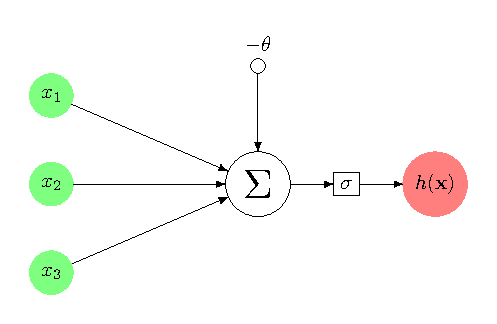
\includegraphics[width=.45\textwidth]{neuron-mp}
  \caption{Neurona McCulloch-Pitts con entrada $\textbf{x}$ y umbral $\theta$.}
  \label{fig:neuron-mp}
\end{figure}

\subsection{Perceptrón}

Con este modelo es posible representar alguna función muy sencilla pero no es útil para aprender funciones con un poco más de complejidad (observamos que el modelo está determinado por $\theta$, un único parámetro libre). Por ello surge una generalización de este modelo llamado el \textbf{perceptrón} \cite{rosenblatt1958perceptron}.

Este modelo incorpora una novedad fundamental: \textbf{pesos} que afectan a las entradas para regular las relaciones y las intensidades de estas. Al establecer conexiones más complejas entre las entradas se consigue que la neurona pueda aprender funciones que no sean tan simples como ocurría con la neurona de McCulloch-Pitts. También se admiten ahora las entradas reales, aumentando el dominio de entrada.

Definimos el perceptrón en \autoref{def:perceptron} y representamos visualmente en \autoref{fig:perceptron} viendo que lo que cambia simplemente son los pesos asociadas a las entradas, que actúan como reguladores de las conexiones.

\begin{definicion}[Perceptrón]
  Sea un vector de entrada $\textbf{x} \in \R^M$ con $M \in \N$, un vector de pesos $\textbf{w} \in \R^n$ y $\theta \in \R$ el umbral de activación, el perceptrón calcula la función $h$ dada por la siguiente expresión:
  $$h(\textbf{x}) = \sigma\left(\sum \limits^M_{i = 1}w_i x_i - \theta\right),$$
  donde $\sigma$ es la función de activación dada por $$\sigma(t) = \begin{cases} 1, \text{ si } t \geq 0, \\ 0, \text{ si } t < 0. \end{cases}$$
  \label{def:perceptron}
\end{definicion}

\begin{figure}[htpb]
  \centering
  %\hspace*{-2.5cm}
  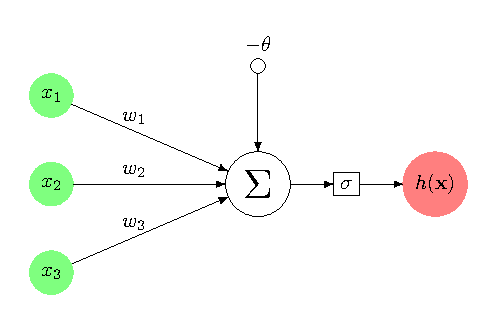
\includegraphics[width=.45\textwidth]{perceptron}
  \caption{Perceptrón con entrada $\textbf{x}$, pesos $\textbf{w}$ y umbral $\theta$.}
  \label{fig:perceptron}
\end{figure}

Considerando $\textbf{x} = (x_1, \ldots, x_M, 1)^T$ y $\textbf{w} = (w_1, \ldots, w_M, -\theta)^T$ podemos compactar la expresión, teniendo entonces $h(\textbf{x}) = \sigma(\textbf{w}^T \textbf{x})$. Observando detenidamente esta expresión vemos que lo que se tiene realmente es un modelo lineal: un \textbf{hiperplano} de $\R^{M}$ al que luego se le aplica una función no lineal.

Sabemos que un hiperplano divide $\R^{M}$ en dos regiones conexas, de manera que la función no lineal lo que está realizando realmente es asignar a cada región un valor distinto. Esta idea tan simple de funcionamiento nos permite pensar que el perceptrón sea capaz de solucionar \textbf{problemas de clasificación binarios}  (\autoref{def:clasbin}).

Estos problemas consisten fundamentalmente en inferir la relación que existe entre los datos de unas variables o \textbf{características} y las \textbf{etiquetas} asociadas a cada dato, que se identifican con una de las dos clases $+1$ o $-1$. Esta relación es la \textbf{función de etiquetado} desconocida $f$ que deseamos aprender, donde sabemos cómo se comporta en una \textbf{muestra} dada y que usaremos para que los modelos puedan aprender una función aproximada $h$. El objetivo entonces se convierte en conseguir que $h \approx f$ (ya veremos adelante como medimos esto).

Como nota adicional si consideramos la muestra extraída $(X, \textbf{y})$, podemos notar que $X \in \mathcal{M}_{N \times M}(\R)$ e $\textbf{y} \in \mathcal{M}_{N \times 1}(\N)$ y que
$$ X = \begin{bmatrix} \textbf{x}_1^T \\ \textbf{x}_2^T \\ \vdots \\ \textbf{x}_N^T \end{bmatrix}, \textbf{y} = \begin{bmatrix} y_1 \\ y_2 \\ \vdots \\ y_{N} \end{bmatrix}.$$

\begin{definicion}[Problema de clasificación binario]
  Sea $M \in \N$ el número de características, y $N \in N$ el número de observaciones, consideramos el espacio $\mathcal{X} \times Y \subseteq R^M \times \{-1, +1\}$ del que obtenemos una muestra $(X, \textbf{y}) \in \mathcal{X}^N \times Y^N$ que sigue una distribución de probabilidad $\mathcal{P}$ desconocida y el espacio de funciones del modelo dado $\mathcal{H}$. El problema consiste en encontrar un $h \in \mathcal{H}$ de tal manera que $h \approx f$, siendo $f$ la función de etiquetado:
  \begin{align*}
    f : \mathcal{X} & \to Y \\
    \textbf{x} & \mapsto f(\textbf{x}) \in \{-1, +1\}.
  \end{align*}
  \label{def:clasbin}
\end{definicion}

Sin más que cambiar los valores de la función de activación $\sigma$ de $\{0, 1\}$ a $\{-1, +1\}$ el perceptrón es capaz de aprender funciones capaces de solucionar estos problemas. De hecho, generalmente en el perceptrón se adopta en vez de la función $\sigma$ anteriormente comentada, la función $\sign$.

Podemos ver que el problema de clasificación binaria es equivalente a encontrar una función que separe dos conjuntos de datos agrupados por la clase, es decir a la separabilidad de dos conjuntos, que es lo que está haciendo el hiperplano $\textbf{w}$ del perceptrón (\autoref{fig:perceptron-ej} \cite{wikipedia2017separ}).

\begin{figure}[htpb]
  \centering
  %\hspace*{-2.5cm}
  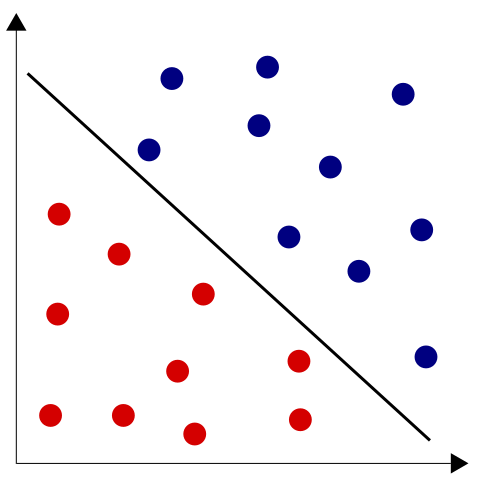
\includegraphics[width=.3\textwidth]{separabilidad}
  \caption{Ejemplo de perceptrón separando linealmente dos conjuntos de datos. Al separar es posible asignar a cada región una etiqueta, siendo equivalente separar a clasificar.}
  \label{fig:perceptron-ej}
\end{figure}

Gracias al Teorema de Convergencia del Perceptrón \cite{novikoff1963convergence} tenemos un resultado fuerte sobre la clase de funciones que puede aprender el perceptrón: se prueba que el modelo es capaz de aprender siempre una función $h$ que separa perfectamente dos conjuntos de datos que sean linealmente separables. Es decir, el perceptrón encuentra una solución muy buena $h \approx f$ ya que coinciden completamente, al menos en la muestra obtenida.

Mediante el \textbf{proceso de aprendizaje} se consigue que el modelo aprenda la función $h$ que buscamos. Este proceso es un método que tiene cada modelo de usar la información de la muestra recogida para poder aprender la función de etiquetado, que en el caso del perceptrón será una simple regla que actualiza los pesos por cada dato de la muestra, dada por
\begin{equation*}
  \textbf{w}_{(t + 1)} =
  \begin{cases}
    \textbf{w}_{(t)}, & \text{si } \sign(\textbf{w}^T_{(t-1)} \textbf{x}_t) \neq y_t, \\
    \textbf{w}_{(t)} + y_t \textbf{x}_t, & \text{en caso contrario.}
  \end{cases}
  \label{eq:percep-rule}
\end{equation*}

A pesar de todo, en cuanto los datos dejan de ser linealmente separables el perceptrón no tiene por qué converger siquiera a una solución. Si bien se puede arreglar quedándose con la mejor solución hasta el momento, las soluciones encontradas no suelen ser muy buenas. Por esta razón se necesitaba encontrar una manera de mejorar este modelo.

\subsection{Perceptrón MultiCapa}

Basándonos \cite{abu2012learning} explicaremos el proceso lógico que se lleva a cabo para poder aumentar la potencialidad del modelo del perceptrón.

Consideremos la siguiente función de la figura (\autoref{fig:xor}, \cite{abu2012learning}) que es bastante simple aunque la función $f$ no se puede aprender con un solo perceptrón (tomando una muestra se ve que los datos no son separables).

\begin{figure}[htpb]
  \centering
  %\hspace*{-2.5cm}
  \includegraphics[width=.35\textwidth]{XOR}
  \caption{Esta $f$ no se puede aprender con un solo perceptrón.}
  \label{fig:xor}
\end{figure}

Usemos dos perceptrones que aprendan cada uno de los hiperplanos separadores (\autoref{fig:dos-percep}, \cite{abu2012learning}) y fijémonos en las áreas de las clases. La función $f$ tiene la clase $+1$ cuando $h_1$ y $h_2$ tienen $(+1, -1)$ ó $(-1, +1)$; y la clase $-1$ cuando $(+1, +1)$ ó $(-1, -1)$. Este comportamiento es análogo a la función booleana $XOR$, por lo que podemos representarla como si lo fuera en base a las salidas de $h_1$ y $h_2$ ($f = XOR(h_1, h_2)$) siendo $+1$ \emph{Verdadero} y $-1$ \emph{Falso}. Usando notación booleana podemos reescribir $f = h_1\overline{h_2} + \overline{h_1}h_2$.

\begin{figure}[htpb]
  \centering
  %\hspace*{-2.5cm}
  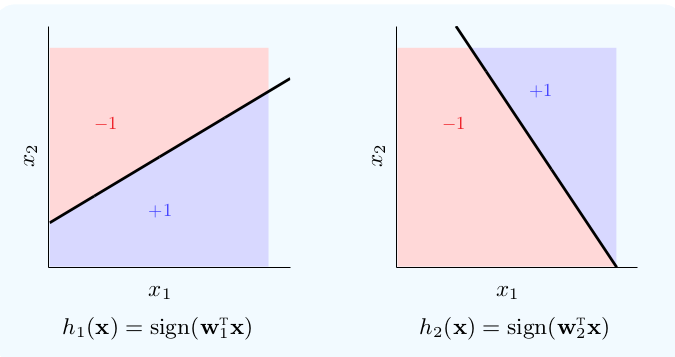
\includegraphics[width=.7\textwidth]{dospercep}
  \caption{Cada perceptrón aprende un hiperplano distinto.}
  \label{fig:dos-percep}
\end{figure}

Como estamos usando funciones $OR (+)$ y $AND (\cdot)$ para obtener $f$, el siguiente paso lógico es intentar expresar estas funciones como perceptrones. Es fácil ver que podemos obtenerlas de la siguiente manera
\begin{align*}
  AND(h1, h2) = \sign(h1 + h2 + 1.5), \\
  OR(h1, h2) = \sign(h1 + h2 - 1.5). \\
  \label{eq:and-or}
\end{align*}

Representamos estas funciones en forma de perceptrones, considerando la forma compacta ($\textbf{x} = (x_1, \ldots, x_M, 1)$, $\textbf{w} = (w_1, \ldots, x_M, -\theta)$ que ya habíamos comentado con la Neurona de McCulloch-Pitts (\autoref{fig:and-or}, \cite{abu2012learning}).

\begin{figure}[htpb]
  \centering
  %\hspace*{-2.5cm}
  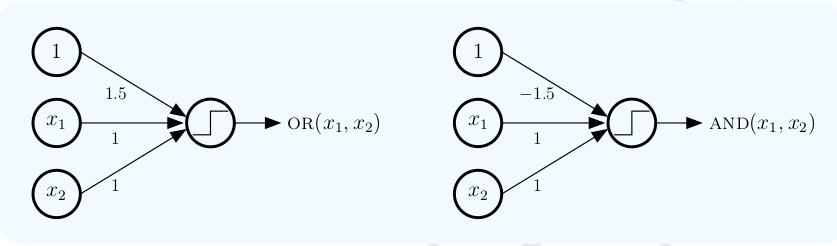
\includegraphics[width=.8\textwidth]{and-or}
  \caption{Funciones $AND$ y $OR$ como perceptrones.}
  \label{fig:and-or}
\end{figure}

Usando estos perceptrones podemos ir implementando poco a poco la función $f$: primero nos encontramos con una $OR$ que tiene como entradas $h_1\overline{h_2}$ y $\overline{h_1}h_2$ (\autoref{fig:or1}, \cite{abu2012learning}).

\begin{figure}[htpb]
  \centering
  %\hspace*{-2.5cm}
  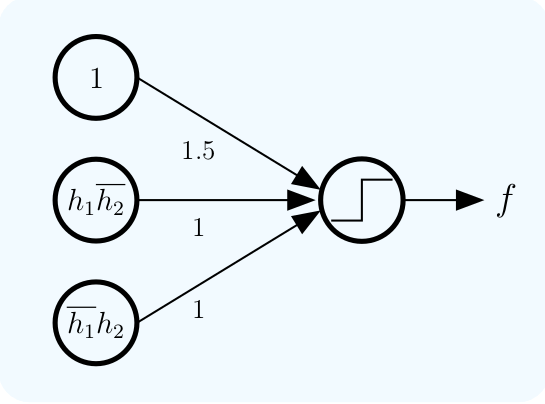
\includegraphics[width=.35\textwidth]{or1}
  \caption{Perceptrón que implementa $AND(h_1\overline{h_2}, \overline{h_1}h_2)$.}
  \label{fig:or1}
\end{figure}

Ahora tendríamos que usar dos perceptrones $AND$ para implementar $h_1\overline{h_2}$ y $\overline{h_1}h_2$. Como ambos perceptrones usarán la misma entrada ($\textbf{h} = (h_1, h_2, 1)$) se pueden representar los dos a la vez mediante dos vectores de pesos distintos (que son lo que determinan al perceptrón). Finalmente hay que tener en cuenta la negación de las entradas que se puede conseguir fácilmente cambiando el signo del peso asociado (\autoref{fig:and2}, \cite{abu2012learning}).

\begin{figure}[htpb]
  \centering
  %\hspace*{-2.5cm}
  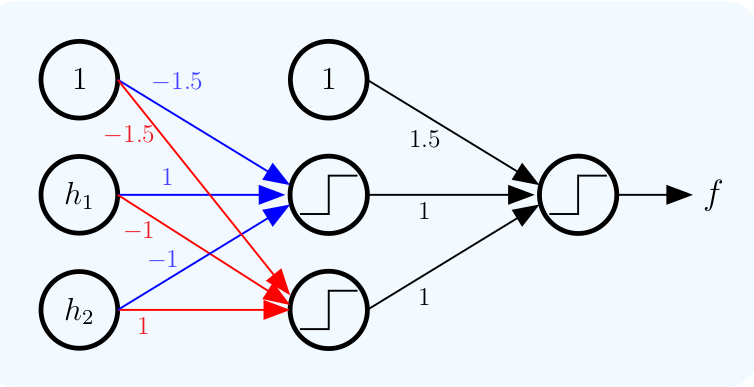
\includegraphics[width=.55\textwidth]{and2}
  \caption{Añadimos dos perceptrones $AND(h_1, \overline{h_2})$ (en azul) y $AND(\overline{h_1}, h_2)$ (en rojo).}
  \label{fig:and2}
\end{figure}

Falta obtener $h_1$ y $h_2$, pero si recordamos que se tenía que $h_1 = \sign(\textbf{w}^T_1 \textbf{x})$ y $h_2 = \sign(\textbf{w}^T_2 \textbf{x})$ que eran los dos perceptrones iniciales. Los incorporamos a nuestro esquema que ya estaría completo (\autoref{fig:mlp}, \cite{abu2012learning}).

\begin{figure}[htpb]
  \centering
  %\hspace*{-2.5cm}
  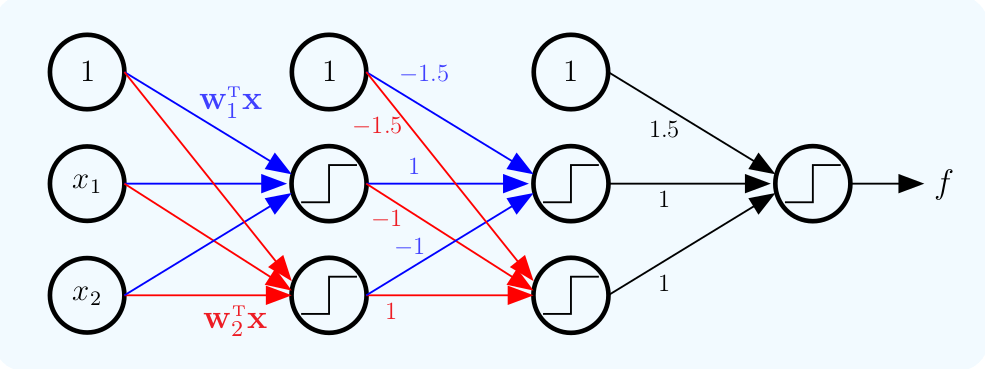
\includegraphics[width=.65\textwidth]{mlp}
  \caption{Los dos perceptrones iniciales $h_1$ (azul) y $h_2$ (rojo).}
  \label{fig:mlp}
\end{figure}

Analizando este modelo vemos que ha sido formado juntando perceptrones, uniendo las salidas de uno con la entrada de otro como si añadiésemos una \textbf{capa} tras otra de perceptrones. Debido a esto, este modelo se conoce como el \textbf{Perceptrón MultiCapa} (\emph{MultiLayer Perceptron}, MLP) \cite{rumelhart1985learning} y es de hecho la primera estructura de red neuronal básica y sobre la que se vertebrará toda la estructura del aprendizaje profundo.

\section{Redes Neuronales Hacia Adelante}

\subsection{Descripción}

Estudiamos las \textbf{redes neuronales hacia delante} (\emph{feedforward neural networks}, FFNN) que son las estructuras de redes neuronales más básicas y funcionales, donde sus procesos de funcionamiento y aprendizaje son el núcleo central de las redes neuronales, por lo que al estudiarlos en detalle nos permitirán entender \emph{a grosso modo} cualquier arquitectura utilizada actualmente.

Como hemos visto, este modelo surge con el perceptrón multicapa que se puede considerar un caso particular de esta aunque también se puede denominar como el mismo tipo de red. Usaremos como base los resultados y explicaciones de \cite{abu2012learning} para detallar exhaustivamente comentando su estructura, algoritmos de cómputo y aprendizaje.

\begin{figure}[htpb]
  \centering
  %\hspace*{-2.5cm}
  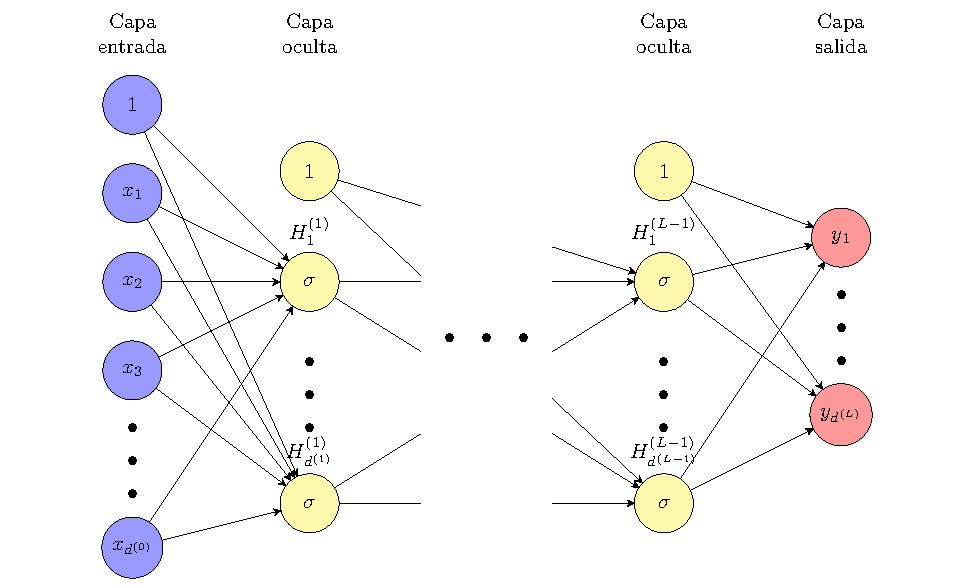
\includegraphics[width=1.\textwidth]{ffnn}
  \caption{Estructura genérica de una FFNN con $L$ capas, dimensiones $d^{(\ell)}$, entrada $\textbf{x}$, salida $\textbf{y}$ y funciones de activación $\sigma$.}
  \label{fig:ffnn}
\end{figure}

\subsection{Estructura}

\subsubsection{Arquitectura}

Veamos primero una estructura general de ejemplo en \autoref{fig:ffnn}. Consideramos una red con $L$ capas, etiquetadas con $\ell = 0, 1, \ldots, L$ donde $\ell = 0$ se corresponde con la capa de \textbf{entrada}, de las variables, que no se suele contar como una capa propia por lo que cuando se dice que una red tiene $L$ capas estamos diciendo que tiene $L-1$ capas intermedias ($0 < \ell < L$), llamadas capas \textbf{ocultas} y la capa $\ell = L$ de \textbf{salida} que es el resultado de la red.

Cada capa tiene una dimensión concreta, que denotaremos por $d^{(\ell)}$ y que indica que la capa $\ell$ tiene $d^{(\ell)} + 1$ nodos o neuronas (incluimos el nodo 1 del sesgo $\theta$) excepto para la capa de salida que se puede obviar. En particular se tiene que $d^{(0)} = M$, el número de variables y que $d^{(L)}$ será la dimensión de la salida, que ya no tiene que ser obligatoriamente un único nodo; de hecho, la salida ya no tiene que tomar valores discretos ya que podemos considerar otras funciones de activación que veremos un poco más adelante.

Observando este diagrama en profundidad notamos que cada neurona de una capa estará conectada por un peso (las conexiones) a todas las neuronas de la siguiente capa, formándose una red \textbf{densa}, nombre por la que también se suele conocer este tipo de capa. Esta estructura de conexiones de entrada a salida, capa por capa, es lo que le da nombre a este tipo de red puesto que los resultados se van pasando \emph{hacia adelante} siempre.

Adicionalmente, tengamos que en cuenta que si cada neurona está asociada con unos pesos, toda la capa $\ell$ que está formada por $d^{(\ell)}$ (sin contar la de sesgo) estará determinada por todos los pesos de cada neurona, que podemos representar como una matriz de la siguiente manera
\begin{equation*}
  W^{(\ell)} = \begin{bmatrix} \textbf{w}^{(\ell)}_{1} \ldots \textbf{w}^{(\ell)}_{d^{(\ell)}} \end{bmatrix} \in \mathcal{M}_{(d^{(\ell - 1)} + 1) \times d^{(\ell)}}(\R).
  \label{eq:pesos}
\end{equation*}

\subsubsection{Función de activación}

Respecto las funciones de activación $\sigma$, también llamadas funciones \textbf{de transformación} ya que son funciones no lineales, se deja de usar la función $\sign()$ en las capas ocultas debido a su discontinuidad en pos de otras funciones aproximadas más \emph{suaves} que realizan una función igual o muy parecida; las más famosas y usadas son las siguientes (funciones dibujadas \autoref{fig:activations}, \cite{moujahid2016activations}):

\begin{enumerate}
  \item Sigmoide: $$\sigma(x) = \dfrac{1}{1 + e^{-x}}.$$
  \item Tangente hiperbólica: $$\tanh(x) = \dfrac{e^x-e^{-x}}{e^{x}+e^{-x}}.$$
  \item ReLU (REctifier Linear Unit): $$ReLU(x) = x^+ = max(0, x).$$
\end{enumerate}

\begin{figure}[htpb]
  \centering
  %\hspace*{-2.5cm}
  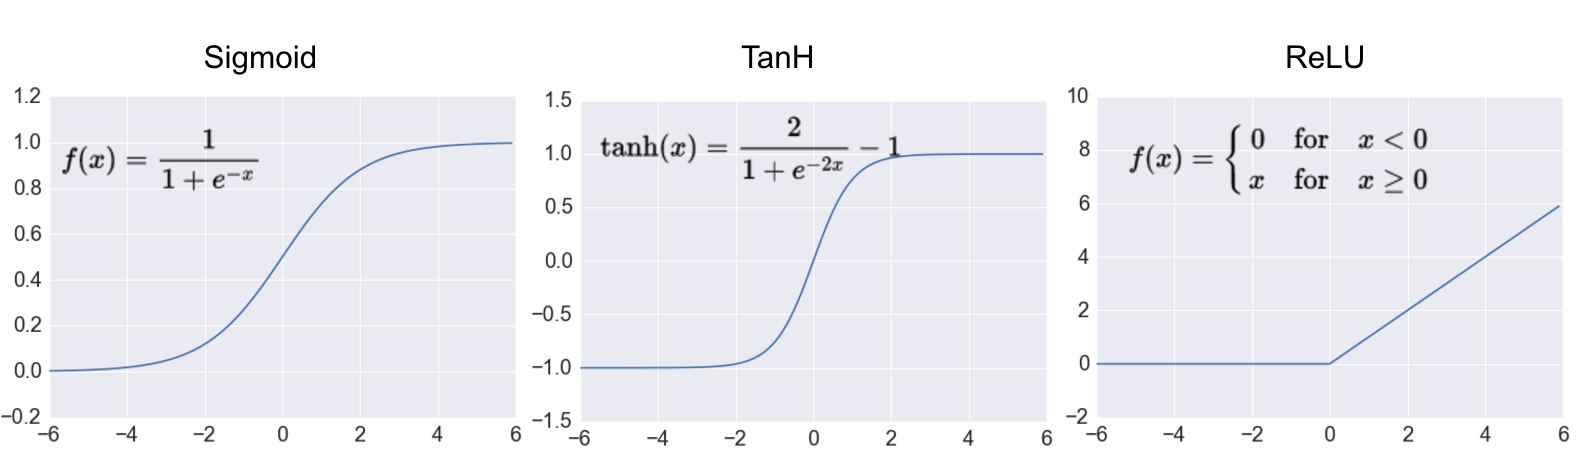
\includegraphics[width=1.\textwidth]{activations}
  \caption{Funciones de activación.}
  \label{fig:activations}
\end{figure}

Donde sí podremos usar $\sign()$ será en la capa de salida cuando queramos obtener un resultado respecto una clase, sin embargo recordemos que ahora podemos tener una dimensión de salida cualquiera y no estamos limitados a aprender funciones discretas. De hecho, si consideramos otras capas de activación para la salida podemos aprender distintos tipos de funciones según el problema que tengamos entre manos.

Por ejemplo, para los problemas de \textbf{regresión} que son simplemente problemas de clasificación donde la $f$ pasa de ser discreta a continua ($f: \mathcal{X} \to Y$, $Y \subseteq \R^n$) podemos usar directamente la función identidad ($f(x) = x$); para los problemas de \textbf{regresión logística}, que considera una función que en vez de asignar una clase directamente asigna la \textbf{probabilidad} ($\mathcal{X} \to Y$, $Y \subseteq [0, 1]$), se puede usar la función $\tanh()$ o \emph{sigmoide}.

De hecho, cuando tenemos un problema de clasificación con $n$ clases en vez de calcular una clase directamente se calcula la probabilidad \textbf{asociada} a cada clase y cuando se hace una clasificación de una única clase se toma la de mayor probabilidad. Esto es posible utilizando en la capa de salida la función de activación \textbf{softmax} \autoref{def:softmax}, que toma un vector real de tamaño $n$ y lo normaliza en una distribución de probabilidad.

\begin{definicion}[Softmax]
  La función softmax es una función $\sigma : \R^n \to \R^n$ definida de la siguiente forma:
  $$\sigma(\textbf{x}) = \sum \limits^n_{i = 1} e^{x_i} \begin{pmatrix} e^{x_1} \\ \vdots \\ e^{x_n}\end{pmatrix}.$$
  \label{def:softmax}
\end{definicion}

En cualquier caso, el modelo $\mathcal{H}_{nn}$ queda determinado por la \textbf{arquitectura} de la red neuronal, es decir, especificar el número de capas y la dimensión de cada capa: fijar $L$ y $\textbf{d} = [d^{(0)}, d^{(1)}, \ldots, d^{(L)}]$. Por tanto cada función de hipótesis $h \in \mathcal{H}_{nn}$ estará representada por los pesos de las conexiones entre las capas que representaremos con matrices: $\textbf{W} = \{W^{(1)}, W^{(2)}, \ldots, W^{(L)}\}$.

\subsection{Propagación hacia adelante}

Antes de explicar el algoritmo de cálculo de $h(\textbf{x})$, indiquemos una breve notación: sea $\ell \in \{1, 2, \ldots, L\}$, consideramos la capa $\ell$ que recibe el el resultado $\textbf{s}^{(\ell)} \in \mathcal{M}_{d^{(\ell)} \times 1}(\R)$ de la multiplicación de la capa anterior mediante la expresión
\begin{equation*}
  \textbf{s}^{(\ell)} = (W^{(\ell)})^T \textbf{x}^{(\ell-1)},
  \label{eq:fp1}
\end{equation*}
usando los datos de entrada $\textbf{x}^{(\ell-1)} \in \mathcal{M}_{(d^{(\ell-1)} + 1) \times 1}(\R)$ con la matriz de pesos $W^{(\ell)} \in \mathcal{M}_{(d^{(\ell-1)} + 1) \times d^{(\ell)}}(\R)$ a los que le aplica la función de activación $\sigma$ obteniendo la salida $\textbf{x} \in \mathcal{M}_{d^{(\ell) \times 1}}(\R)$ dada por
\begin{equation*}
  \textbf{x}^{(\ell)} = \begin{bmatrix} 1 \\ \sigma(\textbf{s}^{(\ell)})\end{bmatrix}.
  \label{eq:fp2}
\end{equation*}

La \textbf{propagación hacia adelante} (\emph{forward propagation}) es el algoritmo para poder calcular el resultado de la red $h(\textbf{x})$. A partir de los datos de entrada $\textbf{x}^{(0)}$ se calcula la siguiente salida de la capa que se \textbf{propaga} a la siguiente capa y así hasta llegar al final siguiendo la siguiente cadena
\begin{equation}
  \textbf{x} = \textbf{x}^{(0)} \xrightarrow[]{W^{(1)}} \textbf{s}^{(1)} \xrightarrow[]{\sigma} \textbf{x}^{(1)} \xrightarrow{W^{(2)}} \ldots \xrightarrow{\sigma} \textbf{x}^{(L)} = h(\textbf{x}).
  \label{eq:cadena-fp}
\end{equation}

Formalizamos este proceso mediante el algoritmo \autoref{alg:fp} \cite{abu2012learning}. Aunque en principio solo necesitamos la última salida $h(\textbf{x}) = \textbf{x}^{(L)}$ devolvemos todas las entradas $\textbf{x'}$ y salidas $\textbf{s}$ ya que los necesitaremos más adelante.

\begin{algorithm}[htbp]
\SetAlgoLined
 \tcp{Inicializamos con la entrada}
 $\textbf{x}^{(0)} \gets \textbf{x}$\;
 \tcp{Propagamos para cada capa}
 \For{$\ell = 1, \ldots, L$} {
  \tcp{Calculamos la entrada de la capa}
  $\textbf{s}^{(\ell)} \gets (W^{(\ell)})^T \textbf{x}^{(\ell - 1)}$\;
  \tcp{Se devuelve la salida de la capa}
  $\textbf{x}^{(\ell)} \gets \begin{bmatrix} 1 \\ \sigma(\textbf{s}^{(\ell)})\end{bmatrix}$\;
 }
 \tcp{Devolvemos las entradas y salidas}
 $\textbf{x'} \gets \left[\textbf{x}^{(0)}, \ldots, \textbf{x}^{(L)}\right]$\;
 $\textbf{s} \gets \left[\textbf{s}^{(1)}, \ldots, \textbf{s}^{(L)}\right]$\;
 \KwResult{$\textbf{x'}$, $\textbf{s}$}
 \caption{$ForwardPropagation(\textbf{x})$)}
 \label{alg:fp}
\end{algorithm}

\subsection{Descenso en gradiente}

Lo último que nos falta para poder empezar a usar estos modelos es un mecanismo de aprendizaje, el algoritmo para que la red pueda aprender la función $f$ mediante la muestra de datos que tenemos, es decir buscar una $h \in \mathcal{H}_{nn}$ tal que $h \approx f$, o lo que es lo mismo $h(\textbf{x}) \approx f(\textbf{x}), \; \forall \textbf{x} \in \mathcal{X}$.

Está claro que cuanto más se aproxime $h$ a $f$ mejor será, aunque necesitamos una manera de formalizar esta similitud para poder trabajarla. Recordemos que tenemos una muestra que podemos suponer que es suficientemente grande y representativa de la distribución subyacente que se puede usar para poder valorar la diferencia entre $h$ y $f$. La idea que surge es valorar con una función de \textbf{error} o \textbf{pérdida} las diferencias entre $f$ y $h$ para todos los valores de la muestra, dando un valor indicativo con el que podemos trabajar.

Este tipo de funciones generalmente son de la forma $E_{\mathcal{D}} : \mathcal{H} \to \R^+_0$ que toman una función del conjunto de hipótesis del modelo y se valora en base a un criterio impuesto según el problema que se quiera resolver usando la muestra $\mathcal{D}$; por ejemplo para problemas de regresión uno querría usar el conocido \textbf{error cuadrático medio}. Fijando una función de error, como queremos la función $h$ que menor $E_{\mathcal{D}}(h)$ tenga el problema de aprendizaje se ha convertido en un problema de \textbf{minimización}, teniendo en cuenta que para que la función sea de variable real tomaremos la representación de $h$ por los pesos $\textbf{w}$ (veremos cómo extenderlo a $\textbf{W}$).

Es importante entender que se puede imponer una función de error para minimizar en un modelo pero que luego el problema original que se quiere resolver sea distinto, de manera que la \textbf{valoración} del modelo se realizará de otra manera; concretamente usaremos las \textbf{métrica} para valorar la bondad de los modelos, que veremos con detalle más adelante en \autoref{ch:metricas}.

Nuestro problema de aprendizaje se ha convertido en un problema de minimización donde para resolverlo podemos recurrir a los métodos numéricos existentes como el \textbf{Descenso en Gradiente} (\emph{Gradient descent}, GD). \cite{curry1944method}.

El descenso en gradiente (\autoref{def:gd}) es un método de minimización cuya idea principal se basa en ir moviéndose hacia el mínimo \emph{bajando} poco a poco tomando la dirección contraria (negativa) del gradiente (\autoref{fig:gd}, \cite{molala2019sd}). Como la dirección del gradiente indica donde aumenta la función localmente, al tomar la dirección contraria después de suficientes iteraciones, esperamos idealmente llegar al menos a un mínimo local (pudiera acabar en puntos de silla) aunque lo deseable será llegar al global si lo hubiera. Bajo ciertas condiciones podemos asegurar la convergencia de este método, por ejemplo si la función es convexa y el gradiente es lipschiziano \cite{shalev2014understanding}.

\begin{figure}[htpb]
  \centering
  %\hspace*{-2.5cm}
  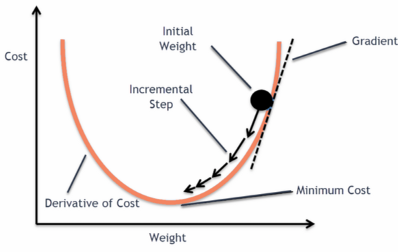
\includegraphics[width=.5\textwidth]{gd}
  \caption{Ejemplo del Descenso en Gradiente en una parábola.}
  \label{fig:gd}
\end{figure}

\begin{definicion}[Descenso en grandiente]
  Sea $E : \R^m \to \R$ una función diferenciable, un punto inicial $\textbf{w}_{(0)}$ y la tasa de aprendizaje $\mu \in \R^+$. El descenso en gradiente es un método iterativo de primer orden para encontrar mínimos que sigue la siguiente regla de actualización:
  $$\textbf{w}_{(t)} = \textbf{w}_{(t-1)} - \mu \nabla E(\textbf{w}_{(t-1)}), \; \forall t \in \N.$$
  \label{def:gd}
\end{definicion}

El establecer un valor para la \textbf{tasa de aprendizaje} (\emph{learning rate}) no es una tarea para nada trivial, de hecho en \autoref{fig:lr} podemos ver las implicaciones de no escoger una tasa adecuada: si es muy baja puede resultar en una convergencia \textbf{muy lenta}, y si es alta puede que \textbf{no converga} o lo haga saltándose mínimos \textbf{mejores}, también podría pasar que el error \emph{explote} (diverge) \cite{ruder2016overview}.

\begin{figure}[htpb]
  \centering
  %\hspace*{-2.5cm}
  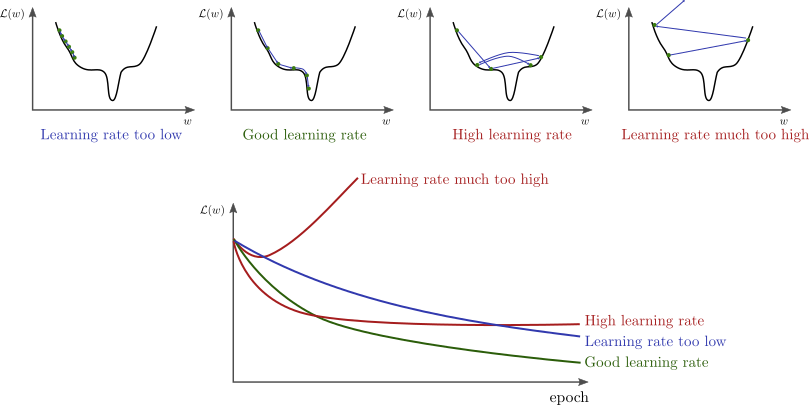
\includegraphics[width=.9\textwidth]{lr}
  \caption{Diferentes resultados según la tasa de aprendizaje $\mu$.}
  \label{fig:lr}
\end{figure}

En principio ya tendríamos un método para poder intentar que nuestra red pueda aprender pero tenemos un problema general a la hora de calcular $\nabla E_\mathcal{D}$: si nuestra muestra de datos $\mathcal{D}$ es muy grande esto puede provocar que el cálculo sea muy costoso en tiempo e incluso supere los tamaños de memoria del \emph{hardware} y esto solo para un paso, por lo que para realizar las múltiples iteraciones necesarias para la convergencia resulte completamente inviable \cite{ruder2016overview}.

La solución a esto la aporta el \textbf{Descenso en Gradiente Estocástico} (\emph{Stochastic Gradient Descent}, SGD) \cite{robbins1951stochastic} que es igual que el Descenso en Gradiente, solo que en vez de tomar todo el conjunto de datos de golpe $\mathcal{D}$ se hace una partición en subconjuntos de tamaño $n$ llamados \textbf{lotes} o \emph{batches} y se actualizan los pesos para cada \emph{batch}. La aleatoriedad que se introduce al escoger los \emph{batches} es interesante ya que nos puede ayudar en la búsqueda de mínimos, aportándonos un poco de exploración para encontrar mejores mínimos en la función.

Técnicamente se llama SGD cuando $n=1$, es decir, cuando actualizamos la red dato a dato, cuando $1 < n < N$ se suele llamar al método \textbf{Descenso en Gradiente con Mini-lotes} (\emph{Mini-batch Gradient Descent}) aunque también se usa SGD indistintivamente.

Respecto al tamaño del \emph{batch} $n$, el rango de valores típico de suele estar en $[32, 256]$ aunque dependerá del modelo y problema concretos que se esté considerando, se suele probar con los valores típicos y se van adaptando para obtener un buen funcionamiento.

En principio ya estaríamos listos para que nuestra red aprendiera, pero merece la pena mencionar que en la actualidad se utilizan métodos derivados más complejos que intentan mejorar el funcionamiento del SGD para una convergencia más rápida y encontrar mejores mínimos. Listamos unos cuantos de los más conocidos y populares: \textbf{Adadelta}, \textbf{RMSprop}, \textbf{Adam}, \textbf{AdaMax} y \textbf{Nadam} \cite{ruder2016overview}. No existe un método absoluto que gane a todos, de hecho SGD sigue siendo una opción viable, por lo que dependiendo del problema se puede decidir escoger uno y otro; aun así uno de los optimizadores más populares y que se suele escoger para las redes neuronales es \textbf{Adam}.

\subsection{Propagación hacia atrás}

\subsubsection{Sensibilidades}

Vamos a aplicar SGD para que nuestro modelo aprenda, para ello necesitamos $\nabla E_{\mathcal{D}} (\textbf{w})$ pero aquí $\textbf{w} = \{W^{(1)}, \ldots, W^{(L)}\}$ por lo que hay que calcular las derivadas parciales respecto \textbf{todas las matrices}. Considerando que el error en la muestra no es más que la media de los errores de cada dato podemos reescribir como
\begin{equation*}
  E_{\mathcal{D}}(\textbf{w}) = \dfrac{1}{N} \sum \limits_{d \in \mathcal{D}} E_d(\textbf{w}) = \dfrac{1}{N} \sum \limits^N_{i = 1} e_i.
  \label{eq:esample}
\end{equation*}

Por tanto las derivadas parciales del error respecto cada matriz de $\textbf{w}$ serán como
\begin{equation*}
  \dfrac{\partial E_{\mathcal{D}}}{\partial W^{(\ell)}} = \dfrac{1}{N} \sum \limits^N_{i = 1} \dfrac{\partial e_i}{\partial W^{(\ell)}}.
  \label{eq:ederiv}
\end{equation*}

Es posible usar métodos numéricos para obtener cada $\dfrac{\partial e}{\partial W^{(\ell)}}$ pero la complejidad del algoritmo para la derivada respecto cada peso sería de $O(Q^2)$ siendo $Q$ el número de pesos, que se hace computacionalmente inviable. Surge así el algoritmo de la \textbf{propagación hacia atrás} (\emph{backpropagation}) que nos permite calcular estas derivadas eficientemente con una complejidad de $O(Q)$.

Este algoritmo se basa en la \textbf{regla de la cadena} para expresar las derivadas parciales de la capa $\ell$ en base a las de la capa $(\ell + 1)$. Para describir el funcionamiento, definamos primero el \textbf{vector de sensibilidad} (\autoref{def:sensibilidad}) que trata de medir como cambia $e$ respecto $\textbf{s}^{\ell}$.

\begin{definicion}[Vector de sensibilidad]
  Sea $\ell \in \N$, el vector de sensibilidad de la capa $\ell$ notado por $\pmb{\delta}^{(\ell)}$, es el gradiente del error $e$ respecto la señal de entrada en la capa $\textbf{x}^{(\ell)}$, es decir:
  $$\pmb{\delta}^{(\ell)} = \dfrac{\partial e}{\partial \textbf{s}^{(\ell)}}.$$
  \label{def:sensibilidad}
\end{definicion}

Usando la regla de la cadena, y recordando que $\textbf{s}^{(\ell)} = (W^{(\ell)})^T \textbf{x}^{(\ell-1)}$ expresamos las derivadas parciales con la sensibilidad de la siguiente forma \cite{abu2012learning}
\begin{equation*}
  \dfrac{\partial e}{\partial W^{(\ell)}} = \dfrac{\partial e}{\partial \textbf{s}^{(\ell)}} \cdot \dfrac{\partial \textbf{s}^{(\ell)}}{\partial W^{(\ell)}} = \textbf{x}^{(\ell - 1)}(\pmb{\delta}^{(\ell)})^T.
  \label{eq:senpar}
\end{equation*}

Además, considerando que $\textbf{x}^{(\ell)} = \sigma(\textbf{s}^{(\ell)})$ y volviendo a aplicar la regla de la cadena podemos obtener la sensibilidad de la capa $(\ell)$ en función de la de $(\ell + 1)$ para cada coordenada
\begin{equation*}
  \delta_i^{(l)} = \dfrac{\partial e}{\partial s_i^{(l)}} =  \sum \limits^{d^{(\ell)}}_{j = 1} \left(\dfrac{\partial e}{\partial s_j^{(\ell + 1)}} \cdot \dfrac{\partial s_j^{(\ell + 1)}}{\partial x_i^{(\ell)}} \right) \cdot \dfrac{\partial x_i^{(\ell)}}{\partial s_i^{(\ell)}} = \sum \limits^{d^{(\ell)}}_{j = 1} \left(\delta^{(\ell)}_i w_{ij}^{(\ell)}\right) \sigma'(s_i^{(\ell)}),
  \label{eq:senpar2}
\end{equation*}
que extendemos al vector entero \cite{abu2012learning}
\begin{equation*}
  \pmb{\delta}^{(\ell)} = \sigma'(\textbf{s}^{(\ell)}) \otimes \left[W^{(\ell + 1)} \pmb{\delta}^{(\ell + 1)}\right]^{d^{(\ell)}}_1,
  \label{eq:senpar3}
\end{equation*}
donde $\otimes$ denota la multiplicación componente a componente y $\left[\empty\textbf{v}\right]^{d^{(\ell)}}_{1}$ indica que se toman las componentes $1, \ldots, d^{(\ell)}$ del vector $\textbf{v}$ que simplemente indica que no contamos la componente del nodo de sesgo (el nodo 1).

Recapitulando: las salidas $\textbf{x}^{(\ell)}$ se pueden obtener simplemente calculando el resultado de la red (propagación hacia adelante), lo que resta por calcular son las sensibilidades $\pmb{\delta}^{(\ell)}$. Replicamos el algoritmo de la propagación hacia adelante con modificaciones: en vez de ir obteniendo y propagando las salidas hacia adelante (se usa $\textbf{x}^{(\ell)}$ para $\textbf{x}^{(\ell + 1)}$), lo haremos con las sensibilidades propagándolas \emph{hacia atrás} (se usa $\pmb{\delta}^{(l+1)}$ para $\pmb{\delta}^{(\ell)}$).

Empezaremos calculando $\pmb{\delta}^{(L)}$ directamente con la definición y después iremos propagando hacia atrás las sensibilidades. Por ejemplo, si consideramos el error cuadrático medio con un modelo cuya salida sea un único valor tendríamos $e(\textbf{x}; h) = (h(\textbf{x}) - y)^2$ y podemos calcular la sensibilidad fácilmente como
\begin{equation*}
  \pmb{\delta}^{(L)} = \dfrac{\partial e}{\partial \textbf{s}^{(L)}} = \dfrac{\partial}{\partial \textbf{s}^{(L)}} (\textbf{x}^{(L)} - y)^2 = 2(\textbf{x}^{(L)} - y) \dfrac{\partial \textbf{x}^{(L)}}{\partial \textbf{s}^{(L)}} = 2(\textbf{x}^{(L)} - y)\sigma'(\textbf{s}^{(L)}).
  \label{eq:delta-ele}
\end{equation*}

Después habrá que calcular la derivada de la función de activación elegida, por ejemplo para $\sigma(s) = \tanh(s)$ tenemos que $\sigma'(\textbf{s}^{(L)}) = 1 - \sigma(\textbf{s}^{(L)})^2$; para la lineal (la identidad) $\sigma(\textbf{s}^{(L)}) = \textbf{s}^{(L)}$ se tendrá simplemente que $\sigma'(\textbf{s}^{(L)}) = 1$.

Describimos el método de \emph{backpropagation} por el cual calculamos las sensibilidades $\pmb{\delta}^{(\ell)}$ en \autoref{alg:bp}.

\begin{algorithm}[htbp]
\SetAlgoLined
 \tcp{Hacemos propagación hacia adelante para obtener $\textbf{x}$ y $\textbf{s}$}
 $\left[\textbf{x}^{(0)}, \ldots, \textbf{x}^{(L)}\right], \left[\textbf{s}^{(1)}, \ldots, \textbf{s}^{(L)}\right] \gets ForwardPropagation(\textbf{x})$\;
 \tcp{Inicializamos las sensibilidades}
 $\pmb{\delta} \gets \dfrac{\partial e}{\partial \textbf{s}^{(L)}}(\textbf{x}, y)$\;
 \tcp{Propagamos hacia atrás}
 \For{$\ell = L-1, \ldots, 1$} {
  \tcp{Calculamos la sensibilidad}
  $\pmb{\delta}^{(\ell)} \gets \sigma'(\textbf{s}^{(\ell)}) \otimes \left[W^{(\ell + 1)}\pmb{\delta}^{(\ell + 1)}\right]^{d^{(\ell)}}_1$
 }
 \tcp{Devolvemos las sensibilidades}
 $\pmb{\delta} \gets \left[\pmb{\delta}^{(1)}, \ldots, \pmb{\delta}^{(L)}\right]$\;
 \KwResult{$\pmb{\delta}$}
 \caption{$BackPropagation(\textbf{x}, y)$}
 \label{alg:bp}
\end{algorithm}

\subsubsection{Aprendizaje}

Por fin podemos definir el algoritmo SGD \autoref{alg:sgd-nn} por el cual podemos hacer que la red aprenda: solo necesitamos pasar como parámetros la muestra $(X, \textbf{y})$, la tasa de aprendizaje $\mu$ y el tamaño de los mini-\emph{batches} $tam_{batch}$. Obviamente se habrá fijado la arquitectura de la red junto a la función de error a minimizar y las funciones de activación.

\begin{algorithm}[htbp]
\SetAlgoLined
  \tcp{Inicializamos los pesos aleatorios}
  $\left[ W^{(1)}, \ldots, W^{(L)}\right] \gets PesosAleatorios()$\;
  \tcp{Iteramos hasta que se cumpla el criterio de parada}
  \Repeat{$CondicionParada()$}{
    \tcp{Dividimos aleatoriamente en mini-\emph{batches} de tamaño $tam_{batch}$}
    $n_{batches} \gets M \, // \, tam_{batch}$\;
    $\left[(X_{1}, \textbf{y}_1), \dots, (X_{n_{batches}}, \textbf{y}_{n_{batches}})\right] \gets ParticionAleatoria(X, \textbf{y})$\;
    \tcp{Por cada mini-\emph{batch} actualizamos los pesos}
    \For{$i = 1, \ldots, n_{batches}$}{
      \tcp{Inicializamos los gradientes a 0}
      $\left[G^{(\ell)}, \ldots, G^{(L)}\right] \gets 0 \cdot \left[W^{(1)}, \ldots, W^{(L)}\right]$\;
      \tcp{Calculamos el gradiente de todo el mini-\emph{batch}}
      \For{$(\textbf{x}, y) \in (X_{i}, \textbf{y}_i)$}{
        \tcp{Forwardpropagation y backpropagation}
        $\left[\textbf{x}^{(0)}, \ldots, \textbf{x}^{(L)}\right] \gets ForwardPropagation(\textbf{x})$\;
        $\left[\pmb{\delta}^{(1)}, \ldots, \pmb{\delta}^{(L)}\right] \gets BackPropagation(\textbf{x}, y)$\;
        \tcp{Actualizamos el gradiente de cada capa}
        \For{$\ell = 1, \ldots, L$}{
          $G^{(\ell)}(\textbf{x}) \gets \textbf{x}^{(\ell-1)}(\pmb{\delta}^{(\ell)})^T$\;
          $G^{(\ell)} \gets G^{(\ell)} + \dfrac{1}{tam_{batch}}G^{(\ell)}(\textbf{x})$\;
        }
      }
      \tcp{Actualizamos los pesos de cada capa}
      \For{$\ell = 1, \ldots, L$}{
        $W^{(\ell)} \gets W^{(\ell)} - \mu G^{(\ell)}$\;
      }
    }
  }
 \tcp{Devolvemos los pesos}
 $\textbf{w} \gets \left[ W^{(1)}, \ldots, W^{(L)}\right]$\;
 \KwResult{$\textbf{w}$}
 \caption{$AprendizajeRed(X, \textbf{y}, \mu, tam_{batch})$}
 \label{alg:sgd-nn}
\end{algorithm}

Esta es la base completa de las redes neuronales, las distintas arquitecturas que se han desarrollado a lo largo de los últimos años no cambian demasiado en los aspectos fundamentales por lo que sabiendo todo lo que hemos visto podemos hacernos una idea de cómo se extiende a los casos más complejos.

\subsection{Error y sobreajuste}

También tenemos que comentar que a la hora de entrenar las redes neuronales hay que tener en cuenta un aspecto fundamental en el aprendizaje automático: el \textbf{compromiso} entre el \textbf{sesgo} (\emph{bias}) y la \textbf{varianza} (\emph{variance}).

Cuando hablamos de sesgo estamos generalmente hablando del error del modelo en el conjunto de nuestra muestra, notado típicamente por $E_{in}$ y en principio es el error que queremos reducir en el proceso de aprendizaje de nuestros modelos. Sin embargo tenemos un problema, si intentamos ajustarnos perfectamente a los datos casi anulando efectivamente el sesgo pudiera ser que en otra muestra distinta de datos observemos que el modelo no ajusta bien estos nuevos datos.

Este efecto es el conocido \textbf{sobreajuste} (\emph{overfitting}) que se da cuando el error de entrenamiento $E_{in}$ no coincide (generalmente es mucho más bajo) con $E_{out}$ que es el error del modelo fuera de nuestra muestra. Este efecto ocurre debido al término de la \textbf{varianza} del error, que para nuestro modelo probablemente sea muy alta, y que nos indica generalmente el grado de variabilidad del error para una muestra distinta de datos.

Cuanto más queramos bajar el sesgo, más nos ajustaremos a los datos y provocaremos que aumente la varianza y por tanto tengamos sobreajuste; si no bajamos el sesgo a costa de no aumentar la varianza entonces el modelo pudiera estar mal ajustado (\emph{underfitting}). Tenemos que encontrar un \textbf{compromiso} entre ambos términos, un equilibrio adecuado para poder alcanzar un buen modelo que resuelva nuestro problema; podemos ver un ejemplo de lo que hablamos en una problema de regresión \autoref{fig:overfitting} \cite{bhande2018overfitting}.

\begin{figure}[htpb]
  \centering
  %\hspace*{-2.5cm}
  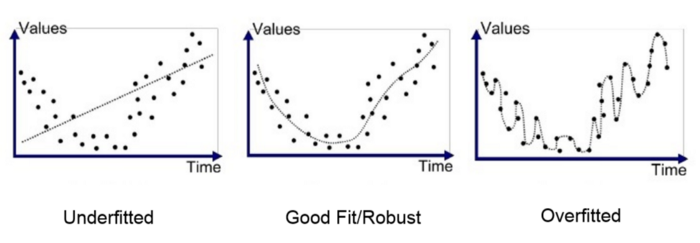
\includegraphics[width=.9\textwidth]{overfitting}
  \caption{Efecto del \emph{overfitting} y \emph{underfitting}.}
  \label{fig:overfitting}
\end{figure}

El proceso del sobreajuste está relacionado con la \textbf{complejidad} del modelo, que nos indica la capacidad del conjunto de hipótesis $\mathcal{H}$ para aprender funciones, siendo una medida común
la \textbf{Dimensión de Vapnik-Chervonenkis} (dimensión VC) $d_{VC}$ \cite{vapnik2015uniform}.  La idea principal es que cuanto más alta es esta dimensión, el modelo es capaz de aprender funciones más complejas y por tanto es capaz de ajustar bien los datos; sin embargo si la complejidad es mucho mayor que la de la función entonces es cuando se produce el efecto del sobreajuste.

Para evitar esto utilizamos técnicas de \textbf{regularización} que se encargan de imponer condiciones sobre el modelo reduciendo así el conjunto de hipótesis $\mathcal{H}$ considerado y disminuyendo su complejidad, que se traduce a un decremento de la varianza a costa de un pequeño aumento del sesgo.

Dentro de este campo hay muchas técnicas que podemos aplicar a las redes neuronales: reducción de la dimensión en profundidad y/o anchura, parada temprana (\emph{early stopping}) que trata de parar el entrenamiento bajo ciertas condiciones, \emph{dropout} \cite{hertz2018introduction, hinton2012improving} que desactiva aleatoriamente algunas neuronas de las capas mientras la red se entrena, o añadir términos de penalización al error (\emph{weight decay}) siendo los más conocidos la regularización L1 (Lasso)
\begin{equation*}
  E_{reg} = E_{in} + \dfrac{\lambda}{N} \sum \limits^{L}_{\ell = 1} ||W^{(\ell)}||_1, \; \lambda \in \R,
  \label{eq:l1}
\end{equation*}
y L2 \cite{krogh1992simple}
\begin{equation*}
  E_{reg} = E_{in} + \dfrac{\lambda}{N} \sum \limits^{L}_{\ell = 1} ||W^{(\ell)}||_2^2, \; \lambda \in \R.
  \label{eq:l2}
\end{equation*}

Para acabar, en las redes neuronales generalmente se deja una muestra de datos que no se usa para entrenar para obtener una estimación del error fuera de la muestra $E_{out}$ que se llama conjunto de \textbf{validación} $E_{val}$ o de \textbf{test} $E_{test}$ y que podemos usar para comprobar si tenemos sobreajuste o no. Si vamos dibujando $E_{in}$ y $E_{val}$ conforme vamos entrenando la red (cada época) podemos observar cuando hay sobreajuste y parar en ese momento (\autoref{fig:overfitting-nn} \cite{julien2018overfitting}).

\begin{figure}[htpb]
  \centering
  %\hspace*{-2.5cm}
  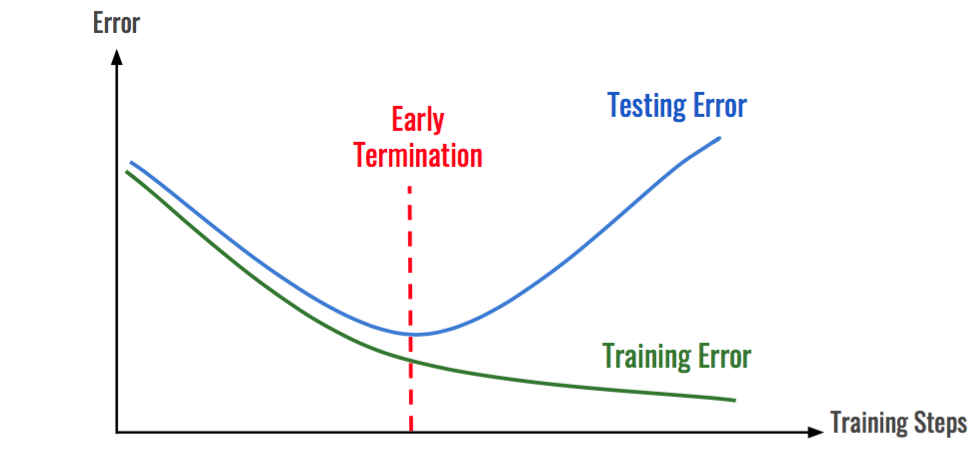
\includegraphics[width=.6\textwidth]{overfitting-nn}
  \caption{Sobreajuste entrenando una red neuronal, tenemos que parar antes de que las curvas diverjan.}
  \label{fig:overfitting-nn}
\end{figure}

\subsection{Teorema de aproximación universal}

Finalmente veamos un resultado matemático que nos permite afirmar con seguridad la fuerte capacidad de las redes neuronales para aprender funciones: el \textbf{teorema de aproximación universal}.

Este teorema tiene dos versiones: el caso de anchura indeterminada, que es la forma clásica, \cite{cybenko1989approximation} y el de profundidad indeterminada \cite{lu2017expressive}.

El caso de anchura arbitraria (\autoref{th:aproxuni-anchura}) nos dice que \textbf{cualquier función continua} en un subconjunto compacto de $R^k$ se puede aproximar con tanta precisión como se quiera con una red neuronal \emph{feed-forward} con una capa oculta y función de activación sigmoide aunque de anchura libre.

\begin{teorema}[Teorema de aproximación universal (anchura indeterminada)]
  Sea $\sigma : \R \to \R$ una función no constante, acotada y continua a la que llamamos función de activación, $I_n$ el hipercubo unidad $n-$dimensional $[0, 1]^n$. Dado un $\epsilon > 0$ y cualquier función $f \in C(I_n)$ entonces $\exists N \in \N$ entero, $\exists \alpha_i, \theta_i \in \R$ constantes reales y $\exists \textbf{w}_i \in \R^n$ vectores reales para $i = 1, \ldots, N$ tal que la función definida como:
  $$F(\textbf{x}) = \sum \limits^N_{i = 1} \alpha_i \sigma \left(\textbf{w}^T_i \textbf{x} + \theta_i \right),$$
  es una realización aproximada de la función $f$, es decir:
  $$|F(\textbf{x}) - f(\textbf{x})| < \epsilon, \; \forall \textbf{x} \in I_n.$$
  En otras palabras, las funciones de la forma $F(\textbf{x})$ son densas en $C(I_n)$. Este resultado también se cumple sustituyendo $I_n$ con cualquier subconjunto compacto de $\R^n$.
  \label{th:aproxuni-anchura}
\end{teorema}

Esta es la versión clásica donde en principio la función $\sigma$ debe ser sigmoide, pero en \cite{leshno1993multilayer} se demuestra que el teorema es cierto para cualquier función $\varphi$ no polinómica. El teorema también se puede extender a cualquier red con profundidad fijada, es decir, con un número de capas ocultas fijo, pero con anchura indeterminada.

Para probar este teorema, primero necesitamos definir cuando una función es \textbf{discriminatoria} \autoref{def:discriminatoria} \cite{cybenko1989approximation}.

\begin{definicion}[Función discriminatoria]
  Sea $M(I_n)$ el espacio de las medidas con signo regulares finitas en $I_n$, una función $\sigma: \R \to \R$ es \textbf{discriminatoria} para una medida $\mu \in M(I_n)$ si:
  $$\int_{I_n} \sigma(\textbf{w}^T \textbf{x} + \theta) d\mu(x) = 0, \; \forall \textbf{w} \in \R^n, \, \forall \theta \in \R \implies \mu = 0.$$
  \label{def:discriminatoria}
\end{definicion}

Ahora probamos el Teorema 1 de \cite{cybenko1989approximation} que es igual que \autoref{th:aproxuni-anchura} pero considerando que $\sigma$ es una función discriminatoria continua.

\begin{teorema}
  Sea $\sigma : \R \to \R$ una función discriminatoria no constante. Dado cualquier $\epsilon > 0$, $f \in C(I_n)$ entonces $\exists N \in \N$ entero, $\exists \alpha_i, \theta_i \in \R$ constantes reales y $\exists \textbf{w}_i \in \R^n$ vectores reales para $i = 1, \ldots, N$ tal que la función definida como:
  $$F(\textbf{x}) = \sum \limits^N_{i = 1} \alpha_i \sigma \left(\textbf{w}^T_i \textbf{x} + \theta_i \right),$$
  es una realización aproximada de la función $f$, es decir:
  $$|F(\textbf{x}) - f(\textbf{x})| < \epsilon, \; \forall \textbf{x} \in I_n.$$
  En otras palabras, las funciones de la forma $F(\textbf{x})$ son densas en $C(I_n)$.
  \label{th:uni1}
\end{teorema}

\begin{proof}
  Sea $S \subset C(I_n)$ el conjunto de funciones de la forma de $F(\textbf{x})$, es trivial que $S$ es un subespacio lineal de $C(I_n)$. Querremos demostrar que la clausura de $S$ es $C(I_n)$.

  Probemos esto por contradicción: supongamos que $R := \overline{S} \neq C(I_n)$ entonces R es un subespacio cerrado propio de $C(I_n)$. Por consecuencia del Teorema de Hahn-Banach (Proposición 3.5 \cite{rudin1973functional}), existe un funcional lineal acotado $L$ en $C(I_n)$ tal que $L \neq 0$ pero $L(R) = L(S) = 0$.

  Por el Teorema de Representación de Riesz \cite{rudin2006real}, este funcional lineal acotado es de la forma
  $$L(h) = \int_{I_n} h(\textbf{x}) d\mu(\textbf{x}), \; \forall h \in C(I_n), \, \mu \in M(I_n).$$

  En particular, como $\sigma(\textbf{w}^T \textbf{x} + \theta)$ está en $R$, $\forall \textbf{w} \in \R^n$, $\forall \theta \in \R$ se debe cumplir que
  $$\int_{I_n} \sigma(\textbf{w}^T \textbf{x} + \theta) d\mu(\textbf{x}) = 0, \; \forall \textbf{w} \in \R^n, \, \forall \theta \in \R.$$

  Sin embargo $\sigma$ era discriminatoria, así que tendríamos que $\mu = 0$  y por tanto $L = 0$ llegando a contradicción. Por tanto, el espacio $S$ debe ser denso en $C(I_n)$.
\end{proof}

Finalmente veamos el Lema 1 de \cite{cybenko1989approximation} que nos dice que las funciones sigmoides continuas son discriminatorias.

\begin{lema}
  Cualquier función sigmoide acotada y medible $\sigma$ es discriminatoria. En particular, cualquier función sigmoide es discriminatoria.
  \label{lema:uni1}
\end{lema}

La demostración de \autoref{th:aproxuni-anchura} queda así demostrada uniendo \autoref{th:uni1} y \autoref{lema:uni1}.

En la otra versión del teorema, de profundidad indeterminada (\autoref{th:aproxuni-prof}), prueba que para toda función Lebesgue-integrable en el espacio de entrada $n$-dimensional respecto la distancia $L^1$ puede ser aproximada por una red neuronal de dimensiones de capa fija $n + 4$ (anchura fija) y función de activación ReLU pero con número de capas ocultas libre.

\begin{teorema}[Teorema de aproximación universal (profundidad indeterminada)]
  Para cualquier función Lebesgue-integrable $f: \R^n \to R$ y cualquier $\epsilon > 0$ existe una red neuronal hacia adelante con función de activación ReLU y anchura $d_m \leq n + 4$ tal que la función $F$ que representa satisface que

  $$\int_{\R^n} |f(\textbf{x}) - F(\textbf{x})| d\textbf{x} < \epsilon.$$
  \label{th:aproxuni-prof}
\end{teorema}

Finalmente cabe añadir que en ambos casos solo se prueba la existencia, no se da una manera para poder construir los pesos ni del tamaño, por lo que el teorema solo nos indica la potencia del espacio de funciones del modelo de las redes neuronales.

\section{Clasificación}

Veamos cómo podemos clasificar las redes neuronales en función del tipo de problema que resuelven o de la arquitectura principal que tienen integrada.

\subsection{Aprendizaje}

Por ser el aprendizaje profundo una subárea del aprendizaje automático, cualquier modelo de red neuronal se puede clasificar atendiendo al tipo de problema que resuelve, donde existen tres ramas principales:

\begin{itemize}
  \item Aprendizaje \textbf{supervisado}: cuando el problema que queremos resolver tiene asociado a los datos unas \textbf{etiquetas}. Se pretende aprender la $f$ desconocida que asigna los datos con las etiquetas mediante la minimización de alguna función de error. Los problemas que ya hemos visto de clasificación y regresión son típicos de aprendizaje supervisado.
  \item Aprendizaje \textbf{no supervisado}: cuando no hay etiquetas, solo nos dan los datos. En este tipo de problemas generalmente se busca patrones y relaciones en los datos, por ejemplo el \textbf{agrupamiento} o \emph{clustering} es un problema típico de aprendizaje no supervisado ya que intenta agrupar los datos en distintos tipos.
  \item Aprendizaje \textbf{por refuerzo}: distinto de los dos anteriores, en estos problemas se intenta enseñar a un modelo como realizar una tarea recompensando o penalizando las acciones que realiza. Crear IAs capaces de jugar al ajedrez, Go o incluso videojuegos entraría dentro de esta categoría.
\end{itemize}

\subsection{Arquitectura}

Veamos aquí distintas arquitecturas con capas más complejas y variadas que han ido surgiendo para intentar abordar problemas de distintos dominios con otros enfoques muy ingeniosos. Obviamos las redes neuronales clásicas que ya hemos explicado y que en cierto sentido podrían considerarse como la red más básica.

\subsection{Redes Neuronales Convolucionales}

Las \textbf{Redes Neuronales Convolucionales} (\emph{Convolutional Neural Networks}, CNN) \cite{lecun1995convolutional} es un tipo de arquitectura orientada al \textbf{tratamiento de imágenes} por lo que se suele usar bastante en problemas cuyos datos sean imágenes de cualquier tipo, en particular prolifera su uso en problemas supervisados de clasificación de imágenes.

Esta arquitectura se basa fundamentalmente en el uso de las \textbf{convoluciones discretas} \autoref{def:convolucion} con las imágenes y un \textbf{tensor} (que puede ser 2D o 3D) denominado \textbf{núcleo} (\emph{kernel}).

\begin{definicion}[Convolución $N$-D discreta]
  Sean dos funciones discretas $f, g : \Z^N \to \R$ definimos la convolución $N$-D discreta de $f$ con $g$ en el punto $\textbf{n} = (n_1, \ldots, n_N)$ como
  $$(f * g)(\textbf{n}) = (f * g)(n_1, \ldots, n_N) = \sum \limits^{+\infty}_{m_1 = -\infty} \ldots \sum^{+\infty}_{m_N = -\infty} f(m_1, \ldots, m_N)g(n_1 - m_1, \ldots, n_M - m_N).$$
  \label{def:convolucion}
\end{definicion}

Esta idea surge de la aplicación de filtros a las imágenes, que se consiguen aplicando estos núcleos convolucionados con la imagen. Los pesos tradicionales que estábamos aprendiendo en las redes se convierten en los valores del núcleo, y lo que se intenta es que la red clasifique imágenes (por ejemplo saber que es un gato o no) \textbf{extrayendo características} que se obtienen al aplicar estos filtros.

Un ejemplo de convolución 2D lo tenemos en \autoref{fig:convolucion-2d} (\cite{pelatrion2020conv}), donde observamos como la convolución realmente es pasar, una matriz en este caso, por la imagen multiplicando coordenada a coordenada y sumando todo el resultado. Esto es extensible fácilmente al caso 3D (\autoref{fig:convolucion-3d} \cite{bansal2018conv}) que es el más usado debido a que las imágenes vienen en 3 canales (RGB) y por tanto pasan de ser matrices (2D) a tensores 3D.

\begin{figure}[htpb]
  \centering
  %\hspace*{-2.5cm}
  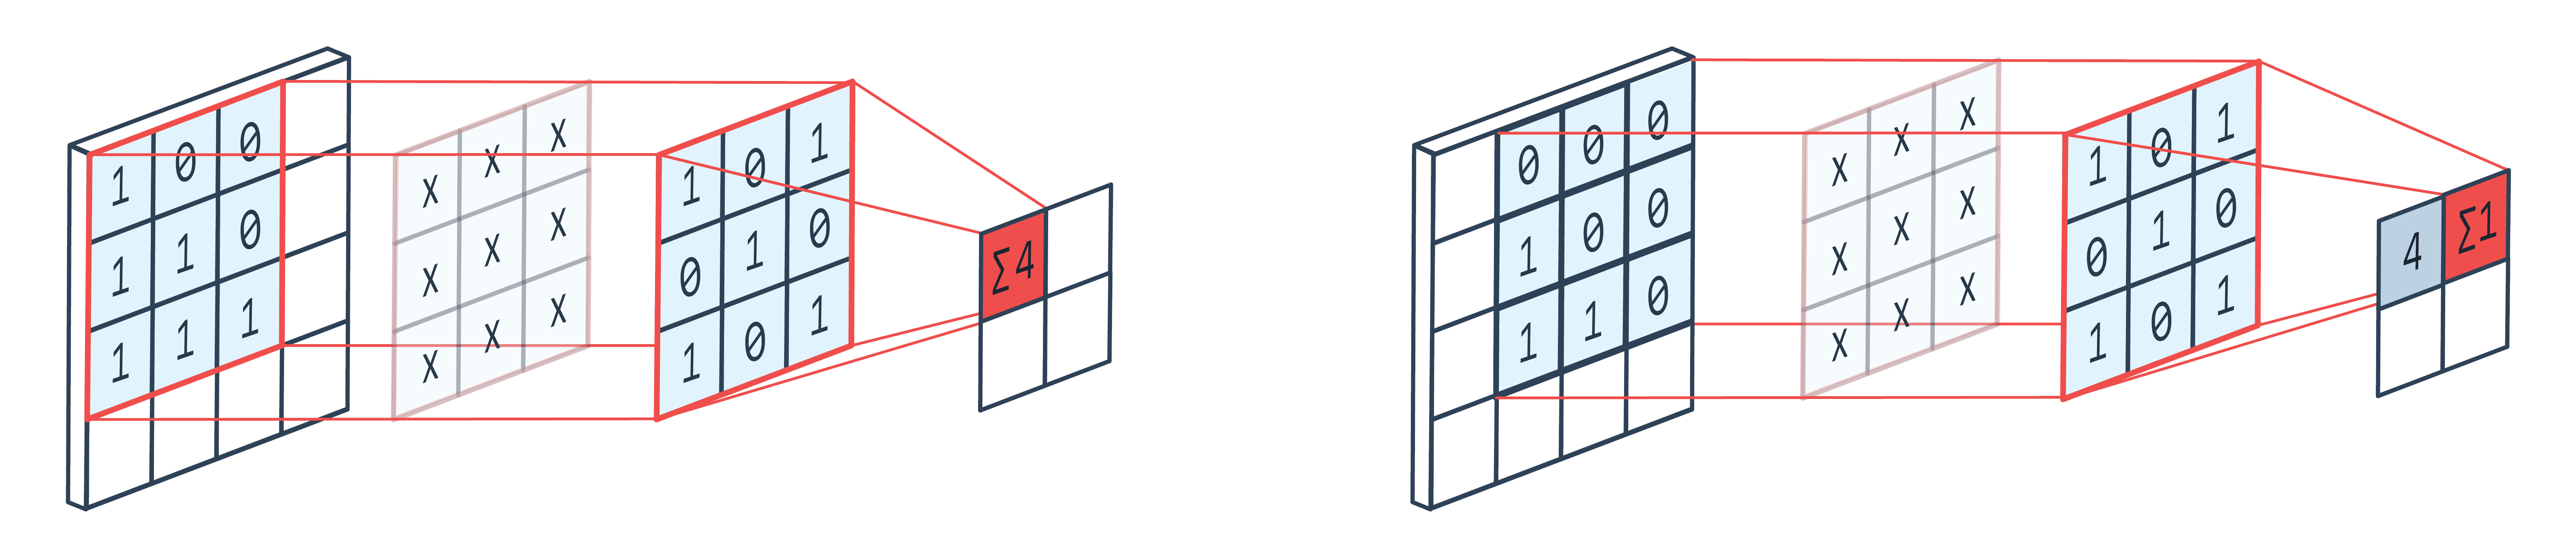
\includegraphics[width=.9\textwidth]{convolucion-2d}
  \caption{Ejemplo de aplicación de convolución 2D.}
  \label{fig:convolucion-2d}
\end{figure}

\begin{figure}[htpb]
  \centering
  %\hspace*{-2.5cm}
  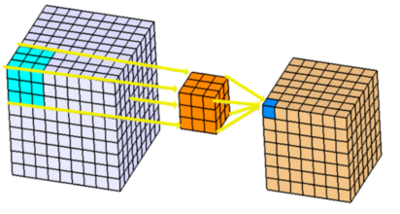
\includegraphics[width=.4\textwidth]{convolucion-3d}
  \caption{Ejemplo de aplicación de convolución 3D.}
  \label{fig:convolucion-3d}
\end{figure}

Notamos que si las imágenes son muy grandes al aplicar diversas capas de filtros el número de pesos puede elevarse bastante y hacerse computacionalmente inviable, por lo que se suele aplicar una técnica de discretización/reducción de dimensión llamada \emph{max-pooling} o \emph{average-pooling }\cite{graham2014fractional}. Esta técnica es igual que aplicar un filtro con $1$ solo que en vez de hacer la suma se toma o bien el máximo o la media de los valores, conseguiendo reducir la dimensión de la imagen tomando representantes de cada área a la que se le aplica; un ejemplo de esto está en \autoref{fig:pooling} \cite{yani2019application}.

\begin{figure}[htpb]
  \centering
  %\hspace*{-2.5cm}
  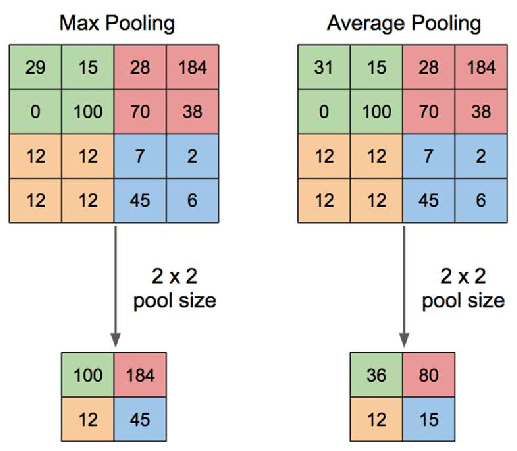
\includegraphics[width=.45\textwidth]{pooling}
  \caption{Ejemplo de \emph{max-pooling} y \emph{average-pooling}.}
  \label{fig:pooling}
\end{figure}

Generalmente la estructura de una CNN tiene dos partes: la primera parte se corresponde al \textbf{extractor de características} que obtiene estas características aplicando filtros mediante el uso de convoluciones con \emph{pooling}, y la segunda es el \textbf{clasificador} que es una red densa (como si fuese una \emph{feed-forward neural network}) que utiliza las características extraídas anteriormente para clasificar las imágenes.

Un ejemplo de esta estructura para clasificar imágenes de dígitos lo tenemos en \autoref{fig:ejemplo-cnn} \cite{saha2018cnn}.

\begin{figure}[htpb]
  \centering
  %\hspace*{-2.5cm}
  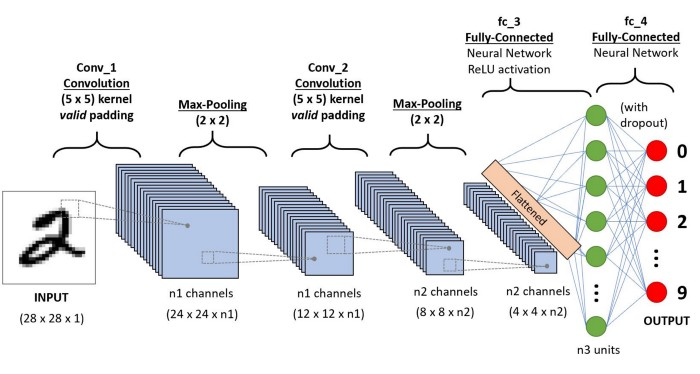
\includegraphics[width=.8\textwidth]{ejemplo-cnn}
  \caption{Ejemplo de estructura de CNN.}
  \label{fig:ejemplo-cnn}
\end{figure}

\subsection{Autocodificador}\label{sec:autoencoder}

Los \textbf{autocodificadores} (\emph{autoencoder, AE}) \cite{mcclelland1986parallel} son redes neuronales modeladas tipicamente para problemas de aprendizaje no supervisado que intentan replicar la entrada en la salida, intentando que en el proceso la red aprenda las características fundamentales de los datos consiguiendo así una \textbf{representación} comprimida de los datos (están codificados).

Veamos la estructura (\autoref{fig:ej-ae}, \cite{sancho2020ae}) que generalmente se divide en dos partes:

\begin{enumerate}
  \item \textbf{Codificador} (\emph{enconder}): la parte de la red que recibe la entrada y va disminuyendo el tamaño de las salidas hasta llegar al vector donde queda codificado la entrada.
  \item \textbf{Descodificador} (\emph{decoder}): la parte de la red que recibe el vector codificador y va aumentado su tamaño hasta llegar a la salida donde reconstruye la entrada original.
\end{enumerate}

\begin{figure}[htpb]
  \centering
  %\hspace*{-2.5cm}
  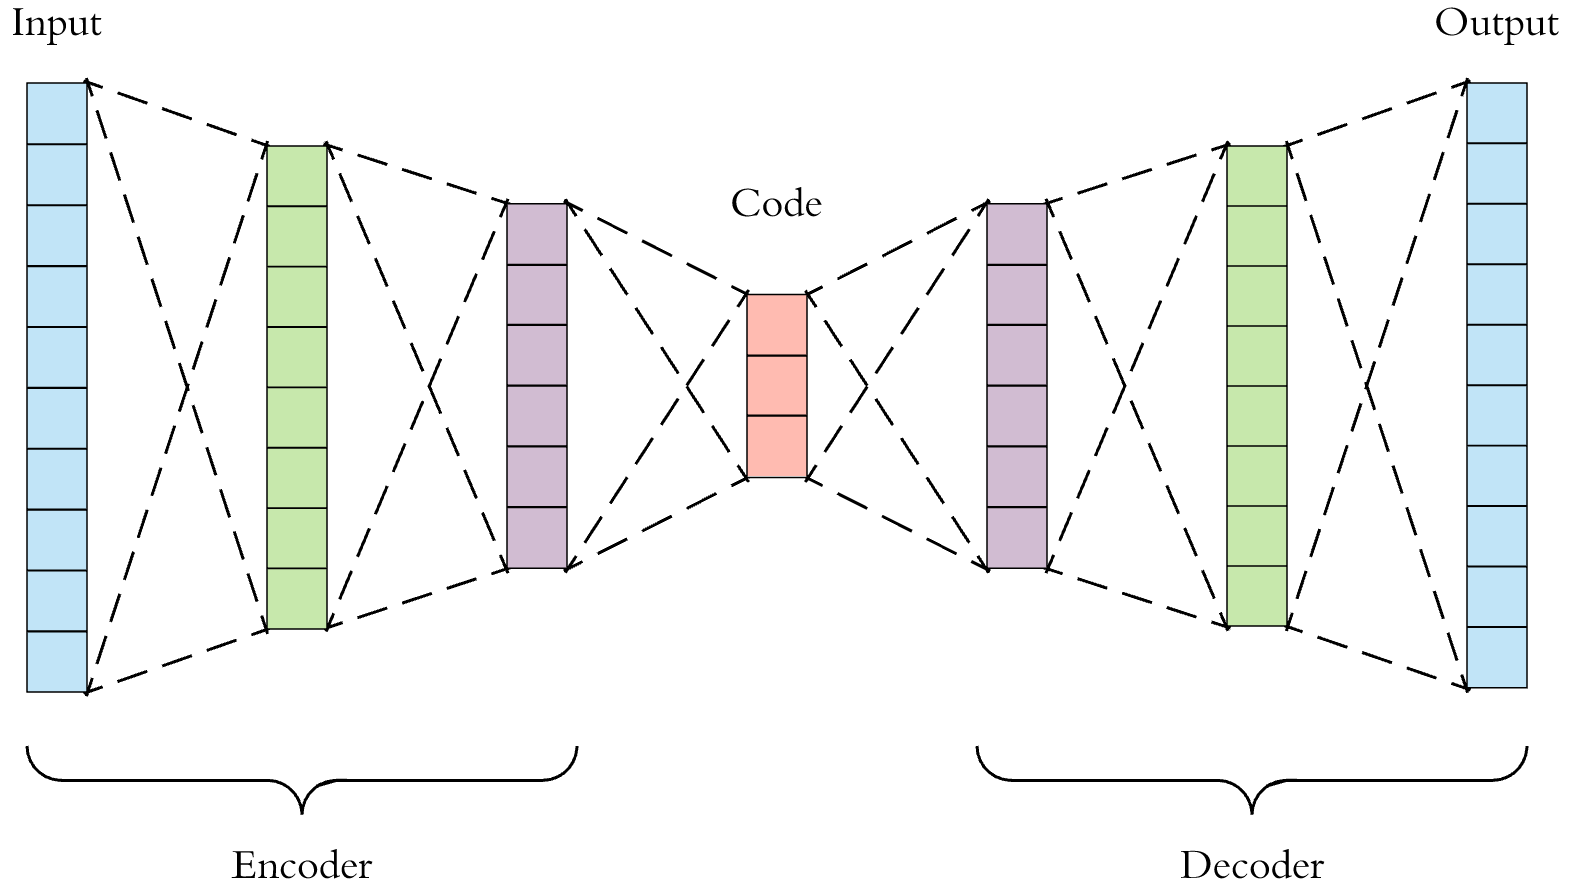
\includegraphics[width=.8\textwidth]{ae}
  \caption{Ejemplo de estructura de un autocodificador}
  \label{fig:ej-ae}
\end{figure}

Este tipo de redes son útiles cuando necesitamos aprender algún patrón o estructura de los datos, o cuando necesitamos comprimir en una dimensión reducida datos muy grandes.

También mencionamos los \textbf{autocodificadores variacionales} (\emph{variational autoencoders}, VAE) que lo que cambian respecto los autocodificadores es el tipo de codificación que se está haciendo, en vez de un vector cualquiera
se busca obtener una representación con \textbf{distribuciones de probabilidad gaussiana}, para ello se toman dos vectores uno de medias $\pmb{\mu} = (\mu_1, \ldots, \mu_n)^T$ y otro de varianzas $\pmb{\sigma}^2 = (\sigma_1^2, \ldots, \sigma_n^2)^T$ de manera que si los juntamos obtenemos un vector de variables aleatorias que siguen distribuciones gausisianas $\mathcal{N}(\pmb{\mu}, diag(\pmb{\sigma}^2))$ de las que podemos obtener una muestra que recontruimos en la salida \autoref{fig:ej-vae} \cite{sancho2020ae}.

\begin{figure}[htpb]
  \centering
  %\hspace*{-2.5cm}
  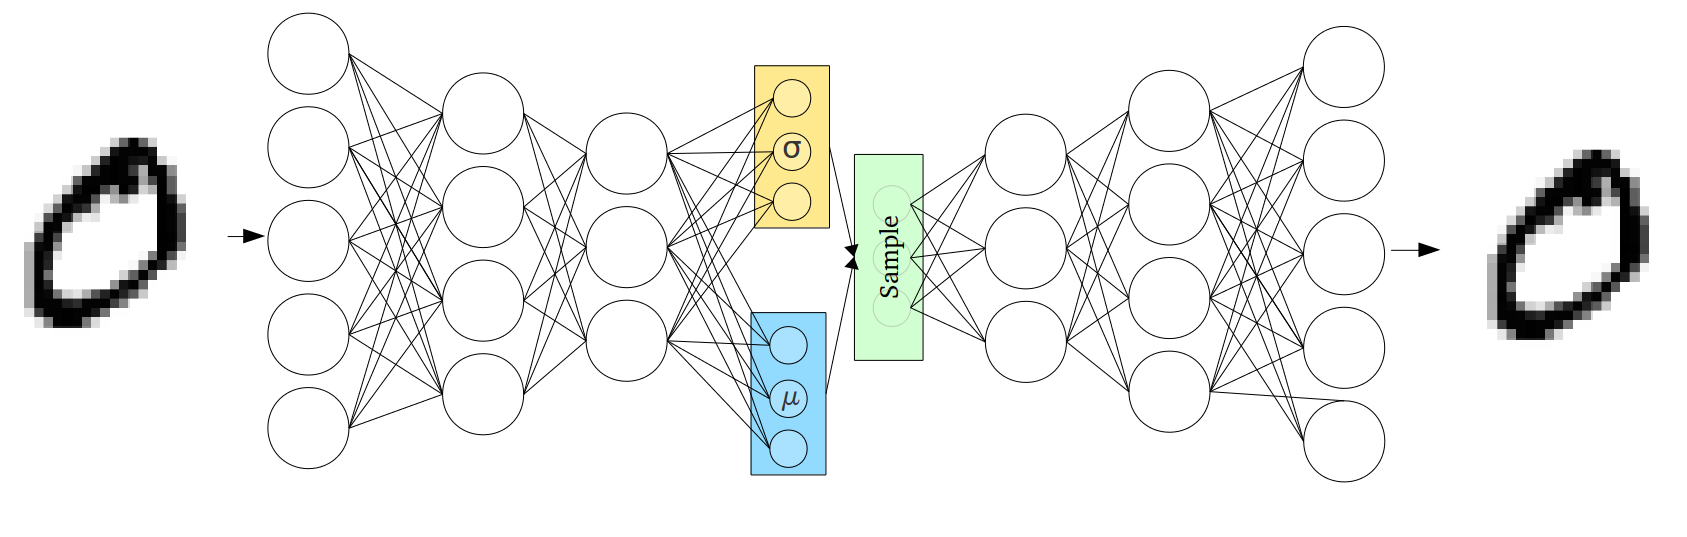
\includegraphics[width=1.\textwidth]{vae}
  \caption{Ejemplo de estructura de un autocodificador variacional}
  \label{fig:ej-vae}
\end{figure}

Para que el entrenamiento se haga correctamente se debe introducir un término nuevo a la función de pérdida que teníamos para la reconstrucción de la entrada: la \textbf{Divergencia de Kullback-Leiber} \cite{kullback1951information} que \emph{a grosso modo} mide la diferencia entre dos distribuciones de probabilidad. Para poder efectuar la diferencia necesitamos saber cual es la distribución latente, pero esta es desconocida así que imponemos la hipótesis de que sea una distribución normal $\mathcal{N}(\textbf{0}, \textbf{1})$ y ya podemos obtener la divergencia como
\begin{equation*}
  D_{KL}(\mathcal{N}(\pmb{\mu}, diag(\pmb{\sigma}^2)) || \mathcal{N}(\textbf{0}, \textbf{1})) = \dfrac{1}{2} \sum^{n}_{i = 1} \left(\sigma^2_i + \mu^2_i - 1 - \log(\sigma^2_i) \right).
  \label{eq:divergencia}
\end{equation*}

Gracias a este diseño, estos modelos son muy útiles para cuando se quieren generar nuevos datos sintéticos que sigan los mismos patrones de los datos donde fueron entrenados, haciendo que parezcan datos auténticos. Por ejemplo podríamos crear un generador de caras en \autoref{fig:caras} \cite{sancho2020ae}.

\begin{figure}[htpb]
  \centering
  %\hspace*{-2.5cm}
  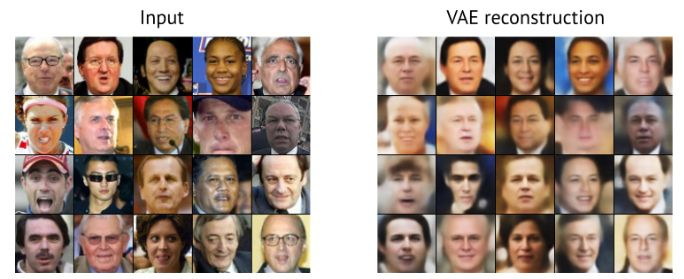
\includegraphics[width=.8\textwidth]{caras}
  \caption{Ejemplo de generador de caras usando un VAE entrenado con caras reales.}
  \label{fig:caras}
\end{figure}

\subsection{Redes Generativas Antagónicas}

Las \textbf{Redes Generativas Antagónicas} (\emph{Generative Adversarial Nets}, GAN) \cite{goodfellow2014generative} es uno de los tipos más novedosos de redes neuronales actualmente cuyo objetivo es crear muestras sintéticas nuevas a partir de una muestra real. Esta arquitectura está compuesta por dos redes distintas: la red \textbf{generadora} (\emph{generator}) y la red \textbf{discriminadora} (\emph{discriminator}). La generadora toma ruido aleatorio como entrada y trata de producir una salida que sea muy parecida a los datos reales, por otro lado la discriminadora toma la entrada del generador y una muestra real del \emph{dataset} y su objetivo es acertar cual es la verdadera (\autoref{fig:gan}, \cite{thalles2018gan}).

\begin{figure}[htpb]
  \centering
  %\hspace*{-2.5cm}
  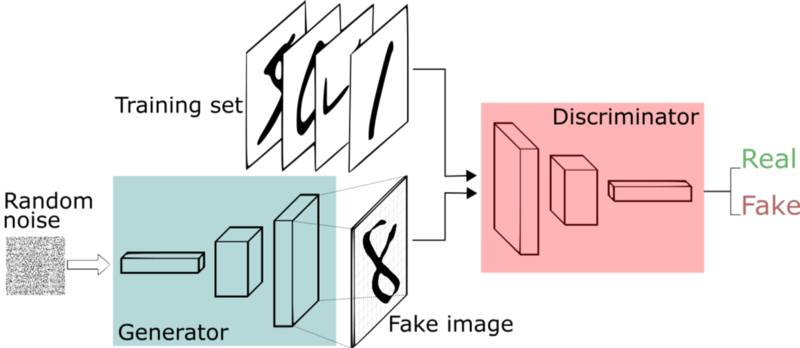
\includegraphics[width=.8\textwidth]{gan}
  \caption{Estructura de una red GAN con dígitos.}
  \label{fig:gan}
\end{figure}

Podemos entender este tipo de red parecido a un juego de suma cero ya que la función de pérdida que intenta minimizar uno es la contraria al otro, por lo que se tiene una especie de \emph{lucha} en el entrenamiento. El generador empieza mejorando los datos fabricados lo que provoca que el discriminador le cueste más diferenciar y se entrene para mejorar su capacidad de discriminación que hace que el generador tenga que hacer mejores fabricaciones; y así cíclicamente, dándonos al final de entrenamiento un generador que devuelve muestras casi imposibles de diferenciar de una real.

Como ya ocurría con los VAE estos modelos son muy útiles para crear datos nuevos que sean prácticamente reales o también para la creación de videos y fotos falsas, modificando las caras de las personas por otras (las famosas \emph{Deepfake} \cite{nguyen2020deepfake}).

\subsection{Redes Neuronales Recurrentes}

Finalmente vemos el tipo de arquitectura en el que nos centraremos, las \textbf{Redes Neuronales Recurrentes} (\emph{Recurrent Neural Networks}, RNN) \cite{elman1990finding} tratan de aprovechar la dependencia temporal que presentan ciertos tipos de datos (frases, música, series temporales...) mediante un flujo de información de entradas anteriores hacia las posteriores (\autoref{fig:rnn-rolled} \cite{christopher2015lstm}).

\begin{figure}[htpb]
  \centering
  %\hspace*{-2.5cm}
  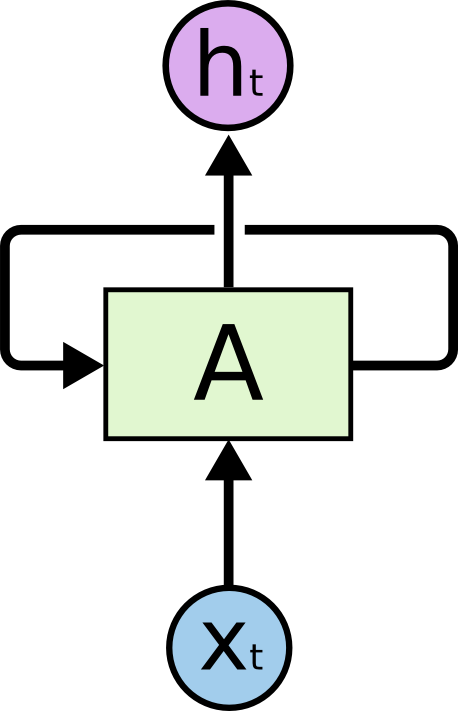
\includegraphics[width=.15\textwidth]{rnn-rolled}
  \caption{Estructura de una RNN.}
  \label{fig:rnn-rolled}
\end{figure}

Esta estructura nos viene a decir que para una cierta entrada $x_t$ el modelo $A$ nos proporciona una salida $h_t$ pero además se pasa a si mismo, retroalimentándose, una información obtenida en función de $x_t$ que se tendrá en cuenta para entradas posteriores ($x_{t + 1}$, $x_{t + 2}$...). Aunque en principio pueda parecer una estructura complicada se puede \emph{desenrollar} en función del tiempo, quedándonos una estructura muy simple (\autoref{fig:rnn-unrolled}, \cite{christopher2015lstm}).

\begin{figure}[htpb]
  \centering
  %\hspace*{-2.5cm}
  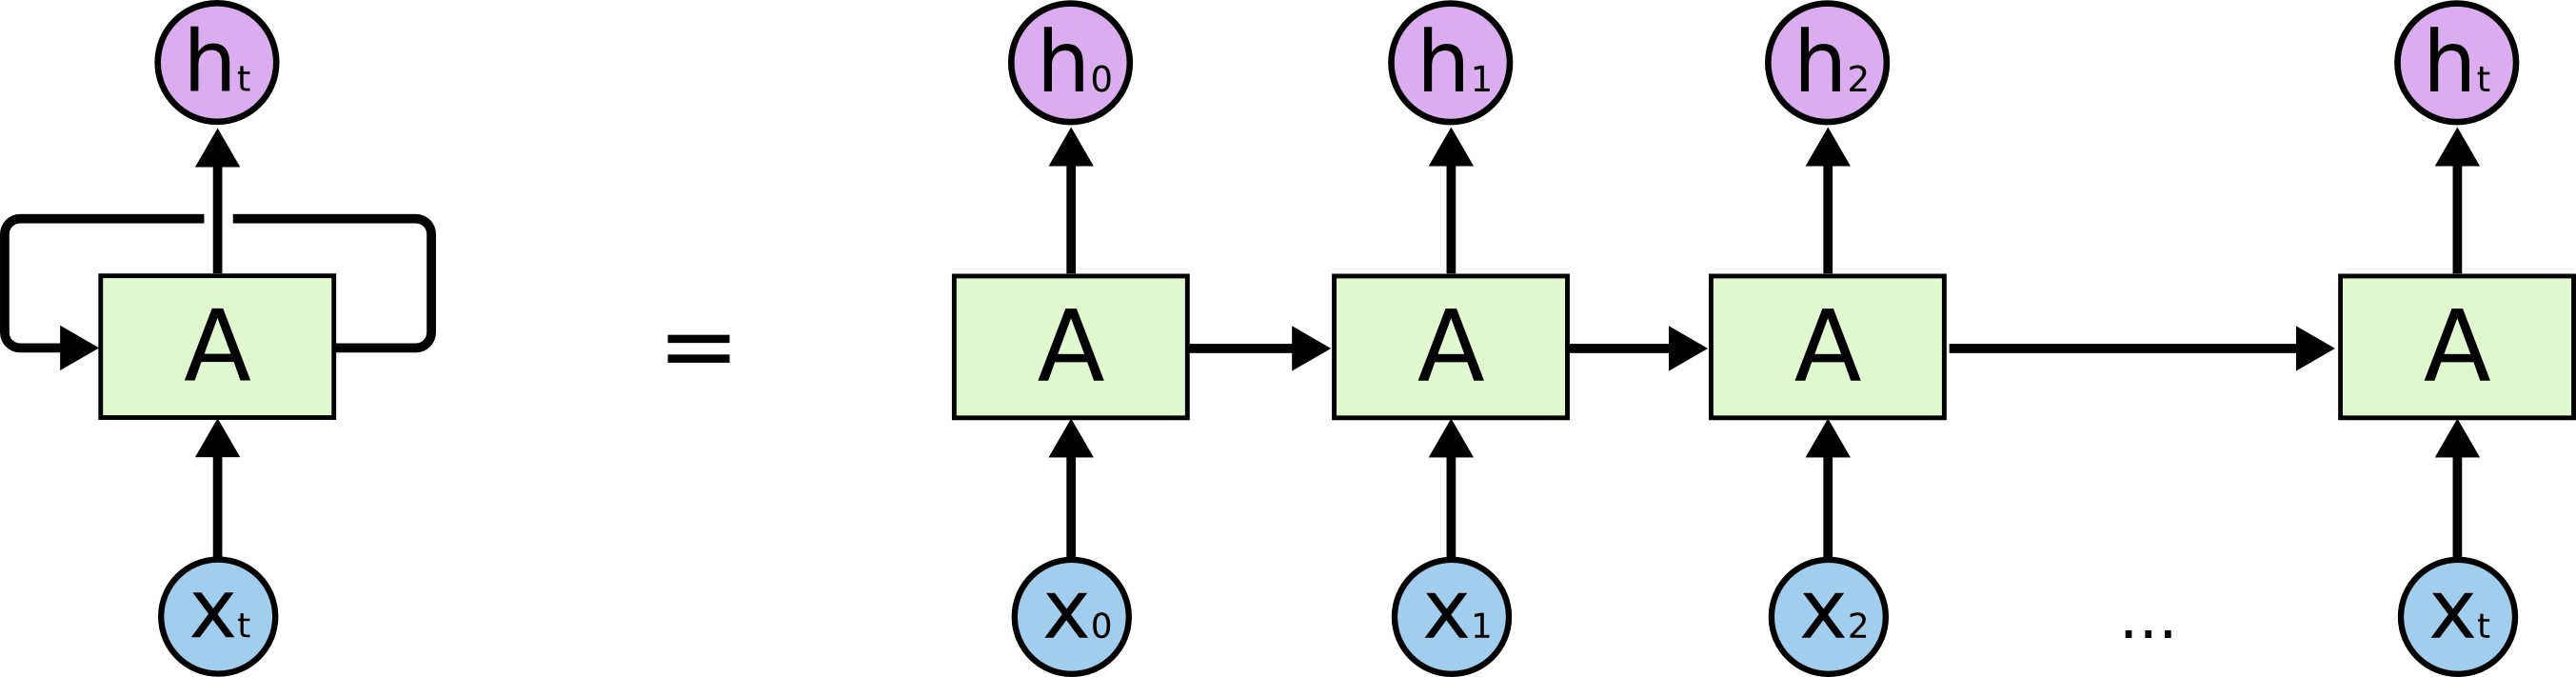
\includegraphics[width=.8\textwidth]{rnn-unrolled}
  \caption{Estructura de una RNN desenrollada.}
  \label{fig:rnn-unrolled}
\end{figure}

Queda claro así cómo según bajo ciertas entradas anteriores, que es lo que proporciona el \textbf{contexto}, la salida de una entrada posterior puede variar enormemente. Así, en las RNN se diseña una neurona especial para enviar la información de manera relativamente sencilla: se une la entrada $x_t$ con la salida de la entrada anterior $h_{t-1}$, que llamaremos \textbf{estado oculto}, a una neurona normal como las conocemos (\autoref{fig:rnn-cells}, \cite{christopher2015lstm}). Tomando como función de activación $\tanh$, La fórmula de cada neurona quedará terminada por los pesos $W$, dada por
\begin{equation*}
  h_t = \tanh \left(W^T \begin{bmatrix} h_{t-1} & x_t & 1 \end{bmatrix}^T\right).
  \label{eq:rnn}
\end{equation*}

\begin{figure}[htpb]
  \centering
  %\hspace*{-2.5cm}
  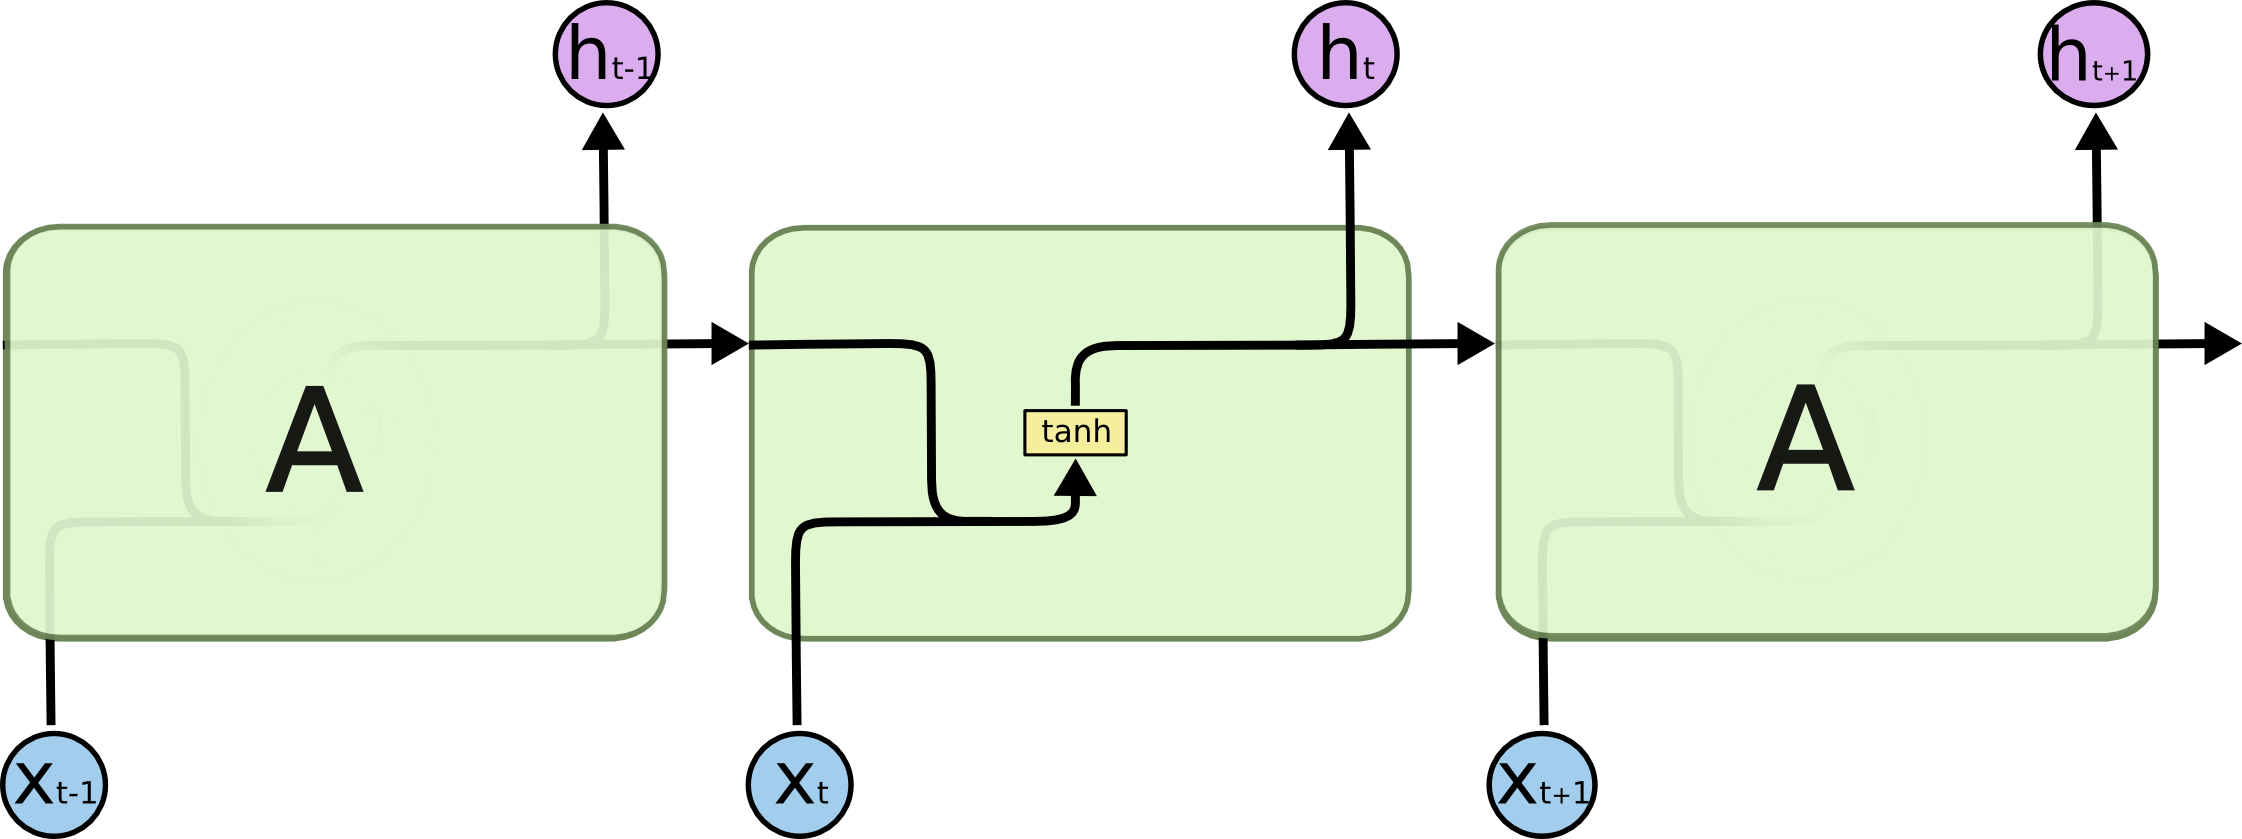
\includegraphics[width=.9\textwidth]{rnn-cells}
  \caption{Estructura de una neurona en una RNN.}
  \label{fig:rnn-cells}
\end{figure}

Sin embargo hay un gran problema: cierta información útil para una entrada \textbf{muy posterior} en el tiempo probablemente no llegue debido a que hay un salto temporal muy grande entre las entradas (\autoref{fig:rnn-longterm}, \cite{christopher2015lstm}), es decir, el modelo no capta bien las \textbf{dependencias temporales a largo plazo} (\emph{long-term dependecies}) \cite{bengio1994learning}.

\begin{figure}[htpb]
  \centering
  %\hspace*{-2.5cm}
  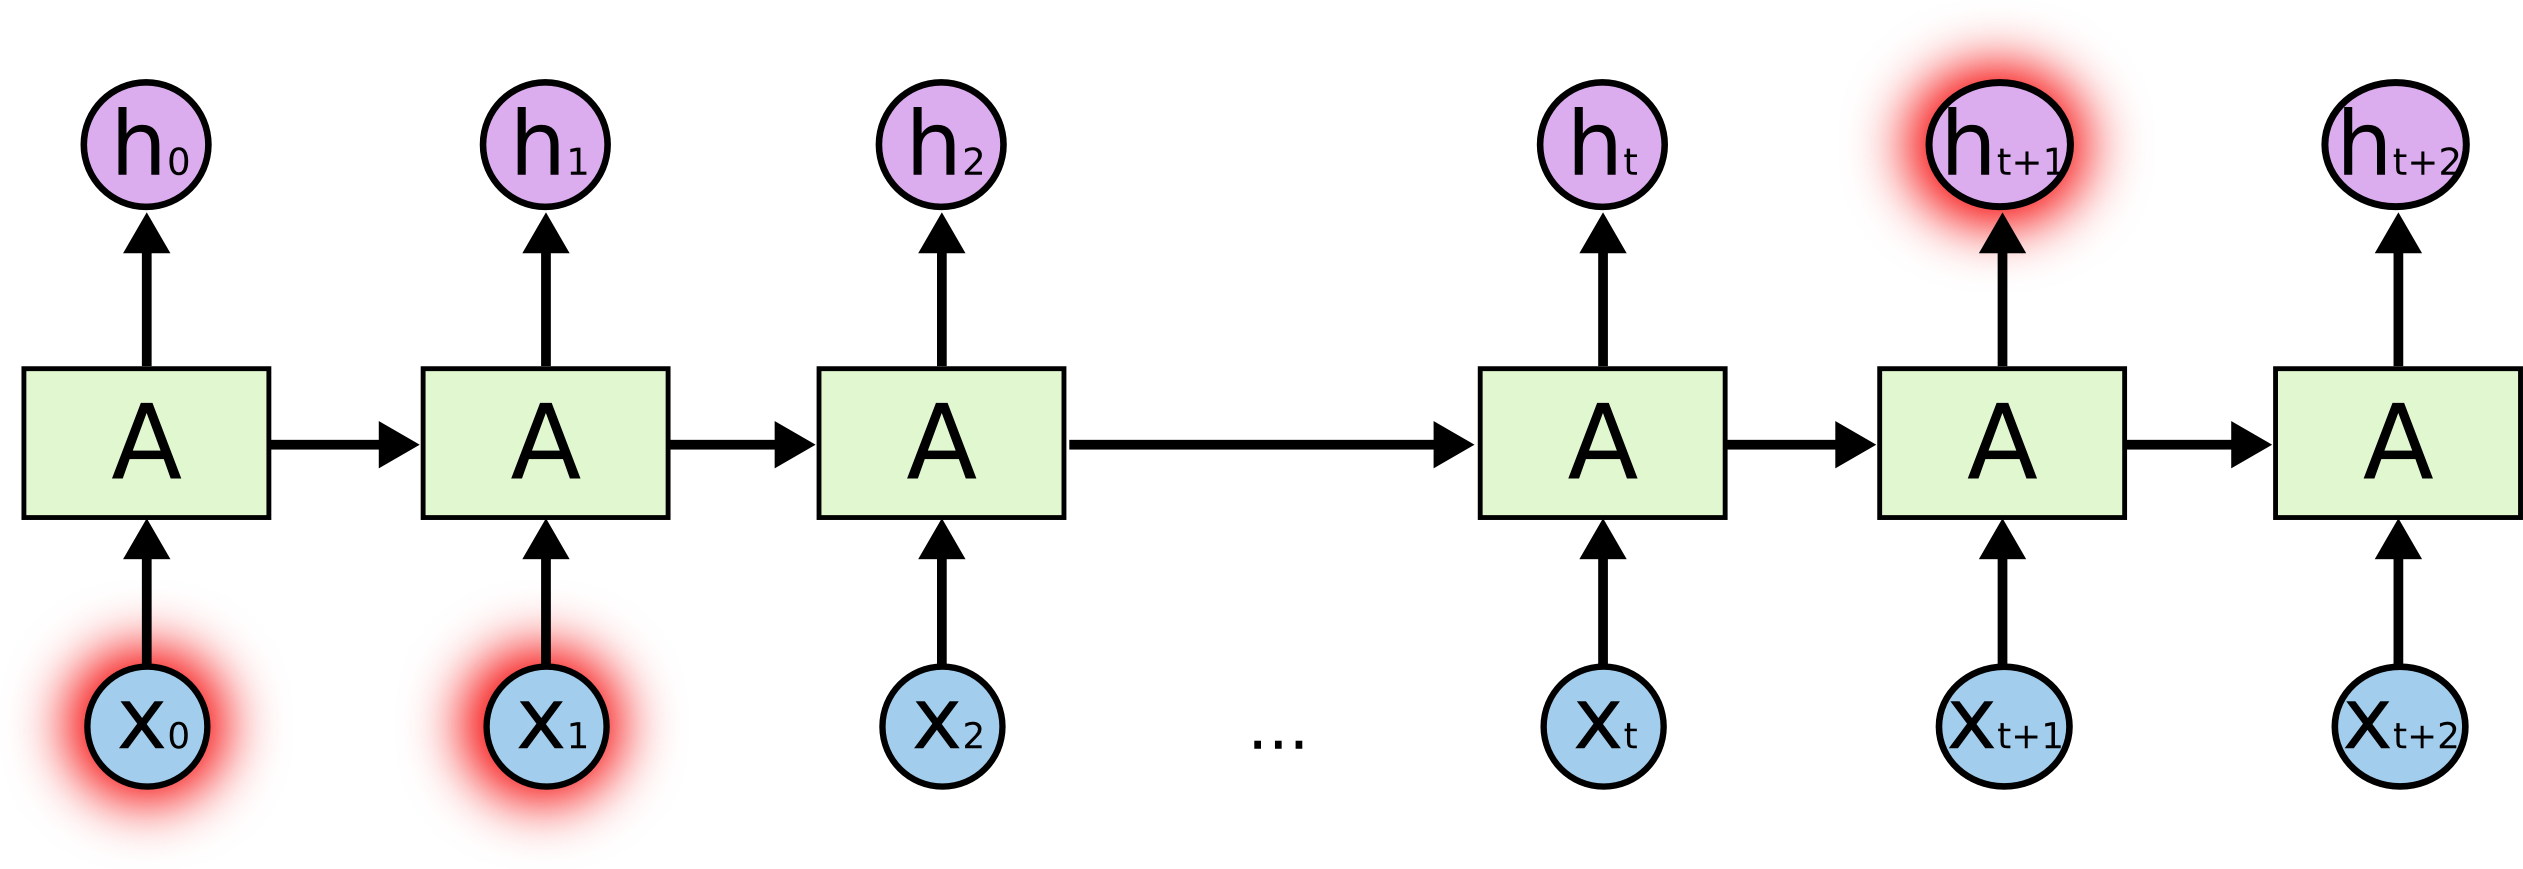
\includegraphics[width=.9\textwidth]{rnn-longterm}
  \caption{La información de $x_1$ y $x_2$ no llega para $h_{t+1}$.}
  \label{fig:rnn-longterm}
\end{figure}

Este obstáculo es consecuencia directa del \textbf{problema del desvanecimiento del gradiente} (\emph{vanishing gradient problem}) que ocurre al entrenar redes neuronales muy profundas, ya que, recordando que para obtener el gradiente íbamos propagando el error desde la última capa hasta la primera capa, el gradiente va disminuyendo poco a poco y si la red es muy extensa entonces va disminuyendo a cero provocando que las capas dejen de actualizarse. Lo que viene a decirnos resumidamente es que la información se pierde rápidamente en el tiempo, por lo que no podemos dar información de entradas muy separadas. También es posible que pase el caso contrario, que el gradiente \textbf{explote} (\emph{explodes}) (aumente hasta valores que sobrepasan el límite de representación de la máquina); en cualquier caso las RNN suelen ser modelos inestables debido a esto \cite{Goodfellow-et-al-2016}.

Para resolver este problema surgen las redes \emph{Long Short Term Memory} (LSTM) \cite{hochreiter1997long}, que consiguen aprender la información tanto a corto como a largo plazo. Estas redes serán las que dedicaremos más atención, y sobre las que nos basaremos para construir nuestros modelos de aprendizaje profundo en el desarrollo del trabajo.

\section{LSTM}

\subsection{Estructura general}

La idea que añade una neurona LSTM para solucionar las dependencias temporales a largo plazo es permitir el paso de la información, recordando u olvidándola, mediante \textbf{puertas} (\emph{gates}) y añadiendo otro flujo de información además del estado oculto $h_t$: el estado celular $C_t$. Este estado intenta emular una especie de \emph{memoria} que irá llevando información relevante desde el principio de la secuencia de entradas hasta mucho más adelante, evitando la pérdida a largo plazo de las RNN.

Primero veamos como está constituida una puerta (\autoref{fig:gate}, \cite{christopher2015lstm}): una neurona normal que recibe una entrada y con función de activación \textbf{sigmoide}, cuya salida realiza una operación de multiplicación coordenada a coordenada con la información que se está regulando. Como la función sigmoide devuelve valores entre $[0, 1]$, al multiplicarlos por la información nos permite, o bien olvidar cuando los valores sean cercanos a 0 ó recordarlos si son cercanos a 1.

\begin{figure}[htpb]
  \centering
  %\hspace*{-2.5cm}
  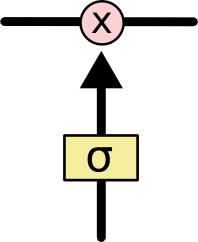
\includegraphics[width=.2\textwidth]{gate}
  \caption{Ejemplo de puerta.}
  \label{fig:gate}
\end{figure}

Fijémonos ahora en la estructura general de una neurona o célula LSTM (\autoref{fig:lstm-cells}, \cite{christopher2015lstm}) y vayamos paso por paso para entender todas los operaciones que tienen lugar. Apreciamos cómo el estado celular viene dado por el flujo superior de la célula, mientras que el estado oculto entra y sale por el inferior y consideramos además que $\sigma \equiv sigmoide$.

\begin{figure}[htpb]
  \centering
  %\hspace*{-2.5cm}
  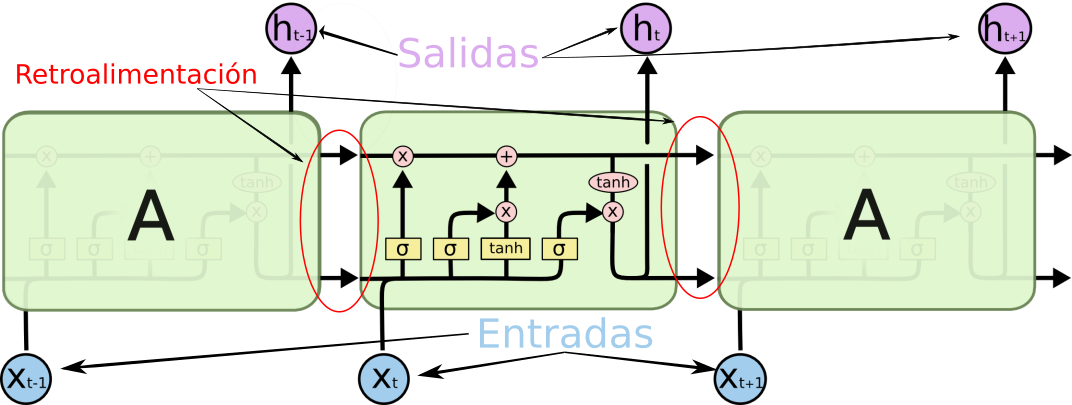
\includegraphics[width=1.\textwidth]{lstm-cells}
  \caption{Esquema de célula LSTM.}
  \label{fig:lstm-cells}
\end{figure}

Primero nos encontramos con la \textbf{puerta del olvido} (\emph{forget gate}), la puerta que se encarga de decidir si la información del estado celular anterior $c_{t-1}$ debería olvidarse o no en base a el estado oculto anterior $h_{t-1}$ y la entrada actual $x_t$; de esta manera controlamos qué información de las variables anteriores recordamos (\autoref{fig:forget} \cite{christopher2015lstm}). El valor de la puerta $f_t$ queda determinado por los pesos $W_f$, en base a
\begin{equation*}
  f_t = \sigma\left(W_f^T \begin{bmatrix} h_{t-1} & x_t & 1 \end{bmatrix}^T \right).
  \label{eq:forget}
\end{equation*}

\begin{figure}[htpb]
  \centering
  %\hspace*{-2.5cm}
  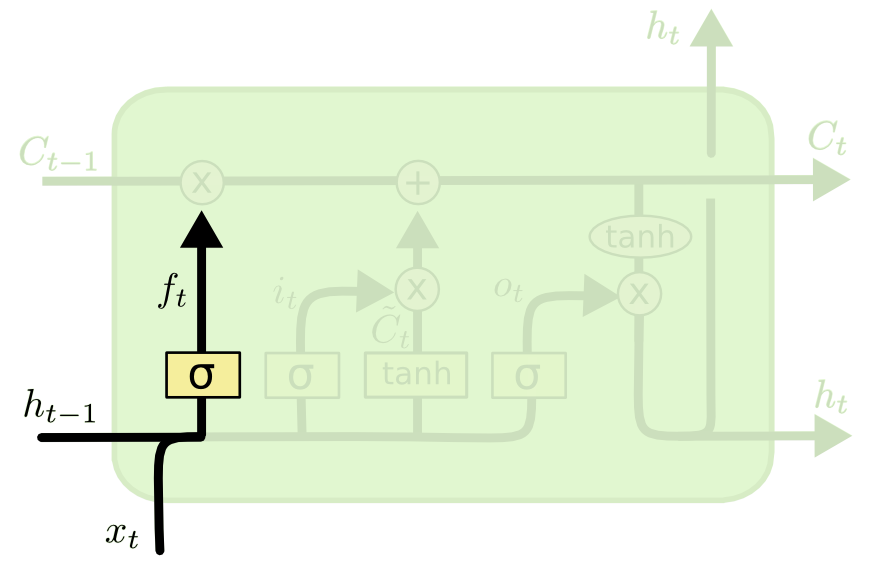
\includegraphics[width=.5\textwidth]{forget}
  \caption{Puerta del olvido $f_t$.}
  \label{fig:forget}
\end{figure}

A continuación tenemos la \textbf{puerta de entrada} (\emph{input gate}) que es la que determina si la nueva información en base a la entrada actual $x_t$ y el estado oculto anterior $h_{t-1}$, se debe incluir o no en el estado celular; indicándonos si esta entrada es relevante o no (\autoref{fig:input} \cite{christopher2015lstm}). Tenemos por un lado el valor de la puerta $i_t$ y el valor de la neurona que tiene la información $\widetilde{C}_t$ donde ambas quedan determinadas por sus pesos $W_i$, $W_{\widetilde{C}}$ con las respectivas fórmulas dadas por
\begin{equation*}
  i_t = \sigma\left(W_i^T \begin{bmatrix} h_{t-1} & x_t & 1 \end{bmatrix}^T\right),
  \label{eq:input1}
\end{equation*}
y
\begin{equation*}
  \widetilde{C}_t = \tanh\left(W_{\widetilde{C}}^T \begin{bmatrix} h_{t-1} & x_t & 1 \end{bmatrix}^T\right).
  \label{eq:input2}
\end{equation*}

\begin{figure}[htpb]
  \centering
  %\hspace*{-2.5cm}
  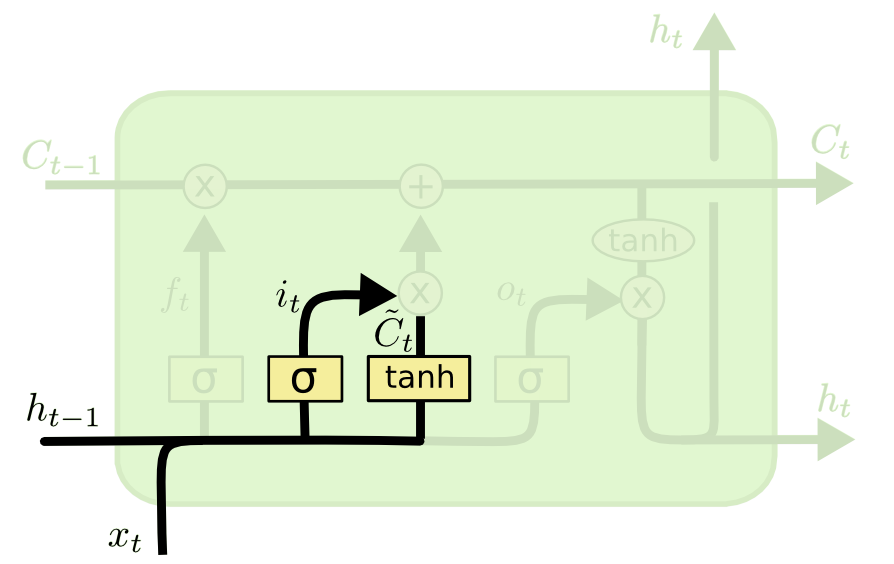
\includegraphics[width=.5\textwidth]{input}
  \caption{Puerta de entrada $i_t$ e información de la neurona $\widetilde{C}_t$.}
  \label{fig:input}
\end{figure}

Llegamos al \textbf{estado celular} que es el valor que lleva la información importante a lo largo de la secuencia y que queda determinada por su entrada anterior $C_{t-1}$ junto a la puerta del olvido $f_t$ y la información actual $\widetilde{C}_t$ junto a la puerta de entrada $i_t$ (\autoref{fig:celular} \cite{christopher2015lstm}). Su valor $C_t$ queda determinada por los valores anteriores en base a la expresión siguiente
\begin{equation*}
  C_t = f_t C_{t-1} + i_t \widetilde{C}_t.
  \label{eq:celular}
\end{equation*}

\begin{figure}[htpb]
  \centering
  %\hspace*{-2.5cm}
  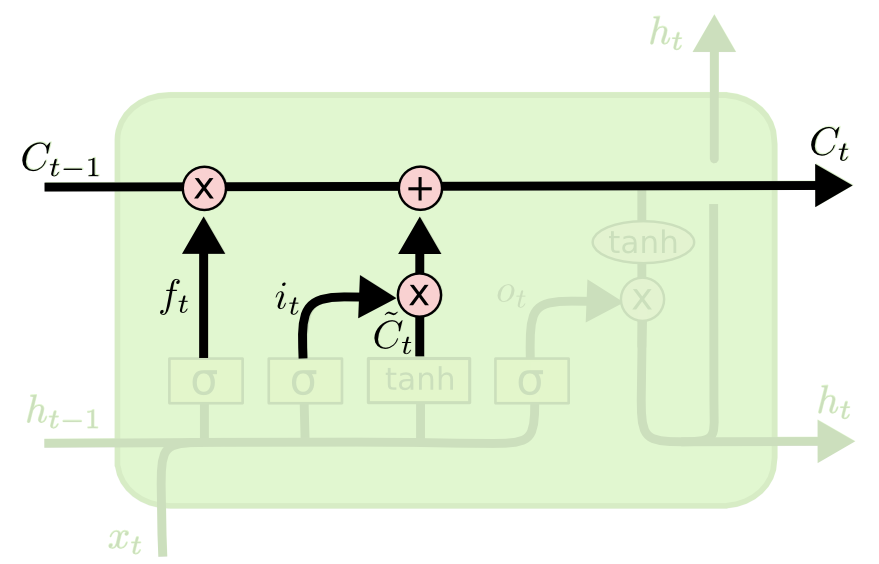
\includegraphics[width=.5\textwidth]{celular}
  \caption{Estado celular $C_t$.}
  \label{fig:celular}
\end{figure}

Finalmente acabamos con la \textbf{puerta de salida} (\emph{output gate}) que regula la información del estado celular $C_t$ que devuelve como salida la célula, es decir, el estado oculto $h_t$ (\autoref{fig:output} \cite{christopher2015lstm}). Tenemos el valor de la puerta $o_t$, determinado por la última matriz de pesos $W_o$, y el estado celular $h_t$ calculados con las respectivas expresiones
\begin{equation*}
  o_t = \sigma\left(W_o^T \begin{bmatrix} h_{t-1} & x_t & 1 \end{bmatrix}^T\right),
  \label{eq:output1}
\end{equation*}
y
\begin{equation*}
  h_t = o_t \tanh\left(C_t\right).
  \label{eq:output2}
\end{equation*}

\begin{figure}[htpb]
  \centering
  %\hspace*{-2.5cm}
  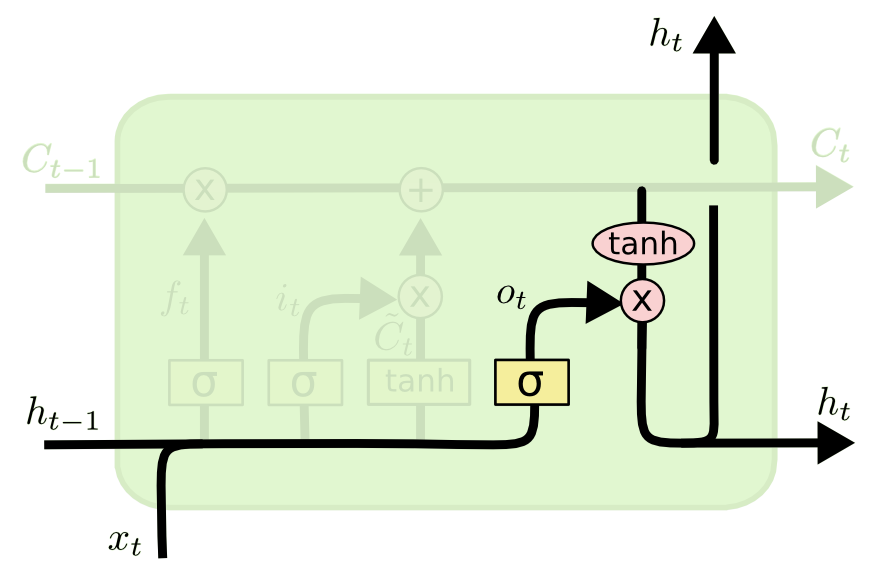
\includegraphics[width=.5\textwidth]{output}
  \caption{Puerta de salida $o_t$.}
  \label{fig:output}
\end{figure}

Observamos que cada célula LSTM tiene 4 neuronas normales con sus pesos respectivos que aprender, siendo de estas 3 para puertas (olvido, entrada y salida) y la cuarta para la información de la propia célula. Este tipo de neurona es mucho más compleja y con muchos mas parámetros libres que aprender que la versión que habíamos considerado en las RNN pero permite flujos de información mucho más ricos al permitir olvidar o memorizar a voluntad y por supuesto que se pueda transmitir información importante desde tiempos muy separados.

\subsection{Variantes}

De esta célula se han creado muchas variantes que generalmente suelen ser modificaciones pequeñas que son ciertamente interesantes. Por ejemplo, \cite{gers2000recurrent} añade conexiones del estado celular anterior $C_{t-1}$ hacia las puertas de manera que los valores quedan actualizados así
\begin{gather*}
  f_t = \sigma\left(W_f^T \begin{bmatrix} C_{t-1} & h_{t-1} & x_t & 1 \end{bmatrix}^T \right), \\
  i_t = \sigma\left(W_i^T \begin{bmatrix} C_{t-1} & h_{t-1} & x_t & 1 \end{bmatrix}^T\right), \\
  o_t = \sigma\left(W_o^T \begin{bmatrix} C_{t-1} & h_{t-1} & x_t & 1 \end{bmatrix}^T\right).
  \label{eq:variante1}
\end{gather*}
obteniendo esta estructura (\autoref{fig:variante1} \cite{christopher2015lstm}).

\begin{figure}[htpb]
  \centering
  %\hspace*{-2.5cm}
  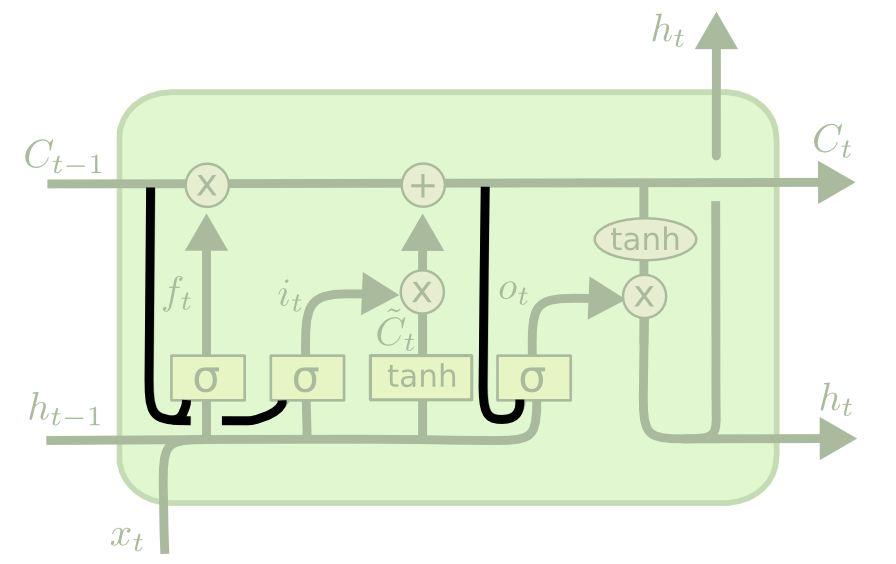
\includegraphics[width=.5\textwidth]{variante1}
  \caption{Variante que introduce cauces de $C_{t-1}$ con las puertas.}
  \label{fig:variante1}
\end{figure}

Otra modificación de \cite{gers2000recurrent} considera unificar las puertas de olvido $f_t$ y entrada $i_t$ de manera que si una puerta considera olvidar la información la otra puerta recuerda; de esta manera solo recordamos algo nuevo si olvidamos lo pasado, y solo recordamos lo pasado si olvidamos lo nuevo (\autoref{fig:variante2} \cite{christopher2015lstm}). Las fórmulas de $C_t$ y $i_t$ actualizadas quedan como
\begin{gather*}
  i_t = 1 - f_t, \\
  C_t = f_t C_{t-1} + (1 - f_t) \widetilde{C}_t.
  \label{eq:variante2}
\end{gather*}

\begin{figure}[htpb]
  \centering
  %\hspace*{-2.5cm}
  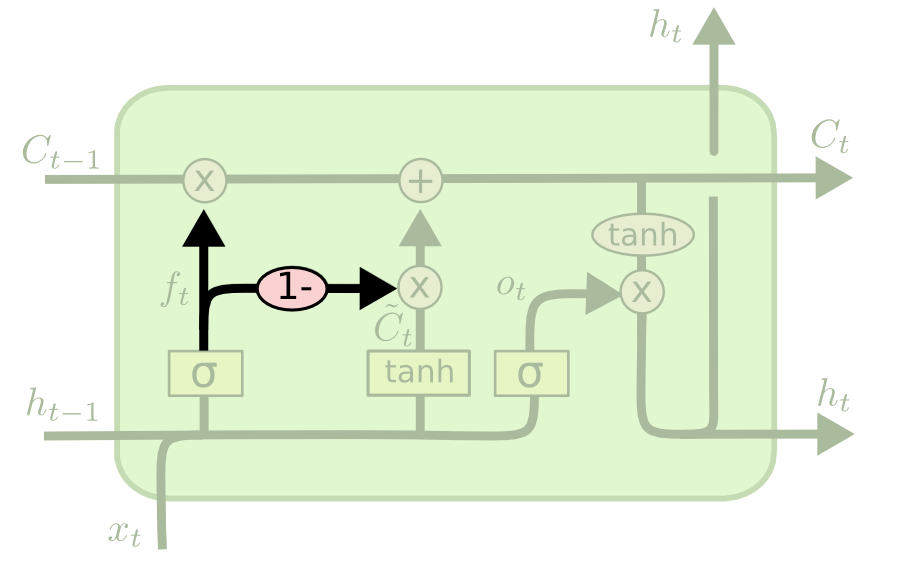
\includegraphics[width=.5\textwidth]{variante2}
  \caption{Variante que sustituye la puerta de entrada por la negación de la del olvido.}
  \label{fig:variante2}
\end{figure}

Finalmente nombramos una de las variantes más conocidas, la \textbf{Unidad Recurrente con Puertas} (\emph{Gated Recurrent Unit}, GRU) \cite{cho2014learning} que intenta simplificar la célula LSTM para reducir los cálculos y conseguir un entrenamiento mucho más rápido mediante la fusión el estado celular con el oculto, así como también las puertas del olvido y de entrada (formando la puerta de actualización $z_t$), quitando la puerta de salida y añadiendo una nueva llamada de reinicio $r_t$. Ahora la célula solo devuelve el estado oculto $h_t$ en función de la siguientes fórmulas
\begin{gather*}
  z_t = \sigma\left(W_z^T \begin{bmatrix} h_{t-1} & x_t \end{bmatrix}^T\right), \\
  r_t = \sigma\left(W_r^T \begin{bmatrix} h_{t-1} & x_t \end{bmatrix}^T \right), \\
  \widetilde{h}_t = \tanh\left(W_{\widetilde{h}}^T \begin{bmatrix} r_t h_{t-1} & x_t \end{bmatrix}^T\right), \\
  h_t = (1 - z_t)h_{t-1} + z_t \widetilde{h}_t.
  \label{eq:gru}
\end{gather*}
junto a la nueva estructura (\autoref{fig:gru}, \cite{christopher2015lstm}).

\begin{figure}[htpb]
  \centering
  %\hspace*{-2.5cm}
  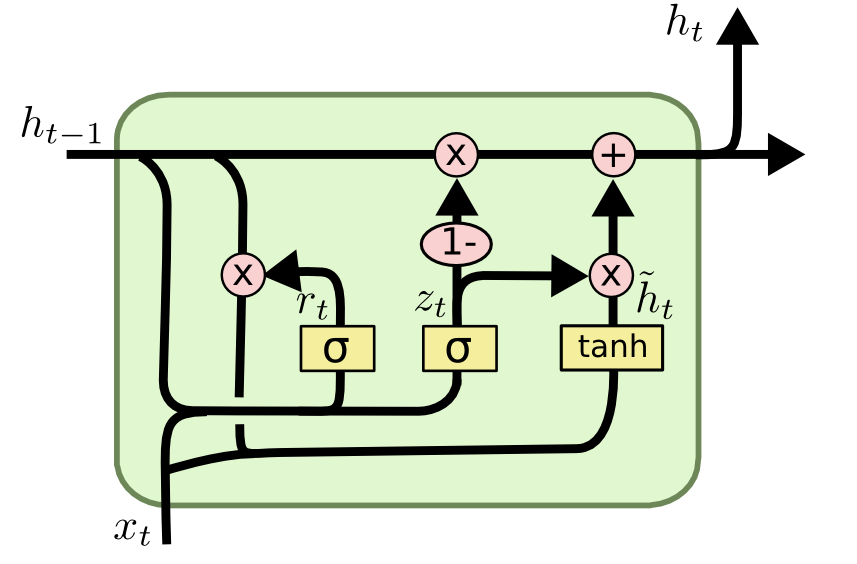
\includegraphics[width=.5\textwidth]{gru}
  \caption{Estructura de la variante GRU.}
  \label{fig:gru}
\end{figure}

Sin embargo, en \cite{greff2016lstm} se hace una comparación de rendimiento entre todas variantes y se observó que no había un modelo que fuese especialmente mejor, todas se comportaban más o menos igual de bien, si bien \cite{gers1999learning} observaron que la versión de LSTM añadiendo un término de error de 1 en la puerta del olvido la hacía la versión más potente de todas las consideradas \cite{Goodfellow-et-al-2016}. Bajo estas razones tomaremos en nuestros modelos las versiones LSTM normales.

\subsection{Recorte}

A pesar de que la arquitectura LSTM evita enormemente el problema del desvanecimiento del gradiente, es posible encontrar en algún caso de entrenamiento que el gradiente explote (la norma del gradiente diverge). Si ocurre esto una técnica muy interesante de utilizar es el método del \textbf{recorte de gradiente} (\emph{clipping gradient}) \cite{pascanu2013difficulty}, que se encarga de ponerle un \emph{tope} a la norma del gradiente cuando supera cierto valor.

Cada vez que se obtiene el gradiente $\textbf{g}$ se aplica la siguiente regla
\begin{equation*}
  \textbf{g}' = \begin{cases} \textbf{g} & \text{si } ||\textbf{g}|| \leq v, \\ v\dfrac{\textbf{g}}{||\textbf{g}||} & \text{en caso contrario,} \end{cases}
  \label{eq:clipping}
\end{equation*}
antes de actualizar los pesos, evitando así que la red use valores enormes del gradiente para actualizar los pesos, haciendo que la red se inestabilice y ya no sirva \cite{Goodfellow-et-al-2016}.

\endinput
